%% The first command in your LaTeX source must be the \documentclass command.
%%
%% Options:
%% twocolumn : Two column layout.
%% hf: enable header and footer.
\documentclass[
% twocolumn,
% hf,
]{ceurart}

%%
%% One can fix some overfulls
\sloppy

%%
%% Minted listings support 
%% Need pygment <http://pygments.org/> <http://pypi.python.org/pypi/Pygments>
\usepackage{listings}
\usepackage{amsmath}
\usepackage{multirow}
\usepackage{graphicx}
\usepackage{caption}
\usepackage{subcaption}
\usepackage{threeparttable}
\graphicspath{ {./img/} }
%% auto break lines
\lstset{breaklines=true}

% \newcommand{\newrev}[1]{{\textbf{{\color{blue}#1}}}}
\newcommand{\newrev}[1]{{{#1}}}

\newcommand{\CellWithForceBreak}[2][c]{
\begin{tabular}[#1]{@{}c@{}}#2\end{tabular}}

%%
%% end of the preamble, start of the body of the document source.
\begin{document}

%%
%% Rights management information.
%% CC-BY is default license.
\copyrightyear{2022}
\copyrightclause{Copyright for this paper by its authors.
  Use permitted under Creative Commons License Attribution 4.0
  International (CC BY 4.0).}

%%
%% This command is for the conference information
\conference{To be decided}

%%
%% The "title" command
\title{Quantifying Knowledge Wealth in Knowledge Graphs: A Case Study of Wikidata}
===> How Quantifying Knowledge Wealth Reveals Knowledge Gap: A Case Study of Wikidata

% \tnotemark[1]
% \tnotetext[1]{You can use this document as the template for preparing your
%   publication. We recommend using the latest version of the ceurart style.}

%%
%% The "author" command and its associated commands are used to define
%% the authors and their affiliations.
\author[1]{TBD}[%
% orcid=0000-0002-0877-7063,
email=tbd@tbd.com,
% url=https://yamadharma.github.io/,
]
% \cormark[1]
% \fnmark[1]
\author[1]{TBD}[%
% orcid=0000-0002-0877-7063,
email=tbd@tbd.com,
% url=https://yamadharma.github.io/,
]
% \cormark[1]
% \fnmark[1]
\address[1]{TBD}

\author[2]{TBD}[%
% orcid=0000-0001-7116-9338,
email=tbd@tbd.com,
% url=https://kmitd.github.io/ilaria/,
]
% \fnmark[1]
\address[2]{TBD}

\author[3]{TBD}[%
% orcid=0000-0002-9421-8566,
email=tbd@tbd.com,
% url=http://conceptbase.sourceforge.net/mjf/,
]
% \fnmark[1]
\address[3]{TBD}

%% Footnotes
% \cortext[1]{Corresponding author.}
% \fntext[1]{These authors contributed equally.}

%%
%% The abstract is a short summary of the work to be presented in the
%% article.
\begin{abstract}
Along with the rapid development of data volumes, the need for machine-readable data is inevitable. As a result, the use of knowledge graph data structures becomes more popular. With its development, quality aspects of a knowledge graph need to be considered, one of which is knowledge wealth: the amount of information contained in a knowledge graph. A high level of knowledge wealth in a knowledge graph may indicate the high quality of a knowledge graph; conversely, a low level of knowledge wealth can be a sign of poor quality of a knowledge graph. However, there is no formal way to define knowledge wealth and how to measure and analyze it. This study proposes a framework to analyze knowledge wealth and the level of knowledge imbalance in the RDF knowledge graph by seeing how the knowledge wealth of an entity class is spread over the knowledge graph using statistical measures and visualization. To evaluate this framework, some use cases were conducted on several classes on Wikidata to detect bias as well as to explore how different definitions of type of wealth impact the magnitude of the Gini coefficient. It is hoped that the results of this study can assist in researching knowledge wealth in the knowledge graph and be used to optimize the efforts of editing and developing knowledge graph projects by the contributors.
\end{abstract}

%%
%% Keywords. The author(s) should pick words that accurately describe
%% the work being presented. Separate the keywords with commas.
\begin{keywords}
  Knowledge graphs \sep
  knowledge wealth \sep
  knowledge imbalance analysis
\end{keywords}

%%
%% This command processes the author and affiliation and title
%% information and builds the first part of the formatted document.
\maketitle


%% include motivating scenario
\section{Introduction}

% To do:
% 1. American researchers: Yang punya property 1, 2, 3, dst itu mereka punya property apa?
% 2. [DONE] Outlier & sample size effect thd gini?
% 3. [DONE] Cek perbedaan 2 entitas di Introduction (pakai query difference) --> + Introduction

% To do (part 2):
% 4. !!! Arsitektural: Library, Flow, etc
% 5. [DONE] Sitasi introduction
% 6. [DONE] Formatting introduction
% 7. !!! Revisi penulisan bias wikidata

% To do (part 3):
% 4. [DONE] Arsitektural: Library, Flow, etc
% 7. !!! Revisi penulisan bias wikidata
% 8. [DONE] Abstrak
% 9. [DONE] Sitasi ke LHKPN: komponen perhitungnan, dan kelas-kelas (pejabat tinggi expected kaya), komponen == jenis kekayaan (perhitungan: by object, by literal, by ID)
% 10. [DONE] Figure 1: caption, kasih summary singkat
% 11. Conclusions
% 12. Bibliografi
% 13. [DONE] Introduction: tambahkan 1 paragraf tentang ide formalisasi, dari contoh yang diberikan. Kaitkan dengan 3 poin kontribusi di paragraf akhir.

% To do (part 3):
% 7. [IN PROGRESS] Revisi penulisan bias wikidata: justifikasi pemilihan class & kasus
% 14. [NEED PLACEHOLDER FOR NOW] link ke Github baru + readme + contoh kode + notebook sederhana buat nunjukin how to pakai (query, visualisasi, stat summary, dll)
% 15. [DONE] autoref subsection S kapital
% 16. [DONE] footnote lhkpn di english
% 17. [DONE] setelah contribution, paper outline: the rest of the paper will discuss ...
% 18. [DONE] discussion: scalability
% 11. !!! Conclusions
% 12. [IN PROGRESS] Bibliografi
% 13. [] All citation bibtex -> Sitasi ke gini formula
% 14. [] Use case: justifikasi kenapa pakai class-class yang disebutkan

% To do (part 4):
% 7. [IN PROGRESS] Revisi penulisan bias wikidata
% 14. [NEED PLACEHOLDER FOR NOW] link ke Github baru + readme + contoh kode + notebook sederhana buat nunjukin how to pakai (query, visualisasi, stat summary, dll)
    %- Python implementation -> nanti notebooknya harus self explanatory, ada comment2 dan step by step apa yang harus dilakukan
% 18. [DONE] discussion: scalability -> tambahan point tentang solution
% 11. !!! Conclusions
% 12. [DONE] Bibliografi
% 13. [DONE] All citation bibtex
% 14. [DONE] Use case: justifikasi kenapa pakai class-class yang disebutkan
    %- justifikasi pemilihan class & kasus
    %- Various kind of occupation, karena representasi di masing2 pekerjaan bisa berbeda2
    %- American: scalability, representative
    %- Western bias: berbeda2 benua 

% To do (part 5):
% 7. [DONE] Revisi penulisan bias wikidata
    %- bagian yang graphical/qualitative, kita tambahkan insight
% 11. [DONE] Conclusions
% 14. [NEED PLACEHOLDER FOR NOW] link ke Github baru + readme + contoh kode + notebook sederhana buat nunjukin how to pakai (query, visualisasi, stat summary, dll)
    %- Python implementation -> nanti notebooknya harus self explanatory, ada comment2 dan step by step apa yang harus dilakukan

% %% include motivating scenario

% (tambahkan 2 paragraf pembukaan)
% distinct - minus = apa yang ada di NYC tapi ga ada di Batam
% Kasih contoh:
% 1. Entitas dengan tipe sama
% 2. Tunjukkan adanya singevalue vs multivalue
% 3. Tunjukkan adanya presence vs absence
% 4. Tunjukkan adanya incoming vs outgoing (incoming itu ga kalah penting, bisa jadi outgoing rendah tapi incoming nya banyak di refer entitas lain)
% 5. Tunjukkan adanya prop type

% contoh lain:
% 1. yang incomingnya banyak
% 2. yang external ID banyak

% Poin:
% 1. ...
% 2. ...

\begin{figure}[!htbp]
    \centering
    % 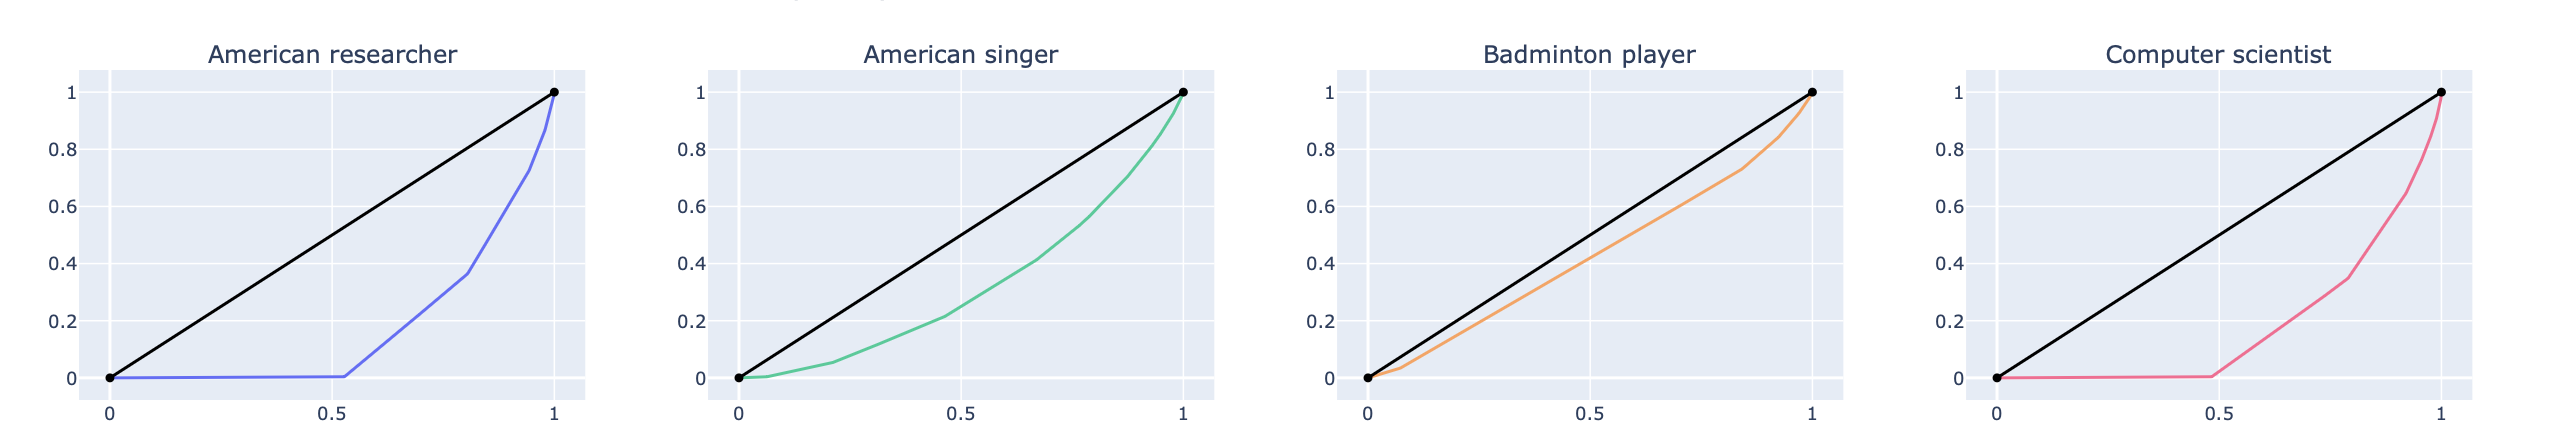
\includegraphics[scale=.5]{Gini - Pure Literal}
    \makebox[\textwidth][c]{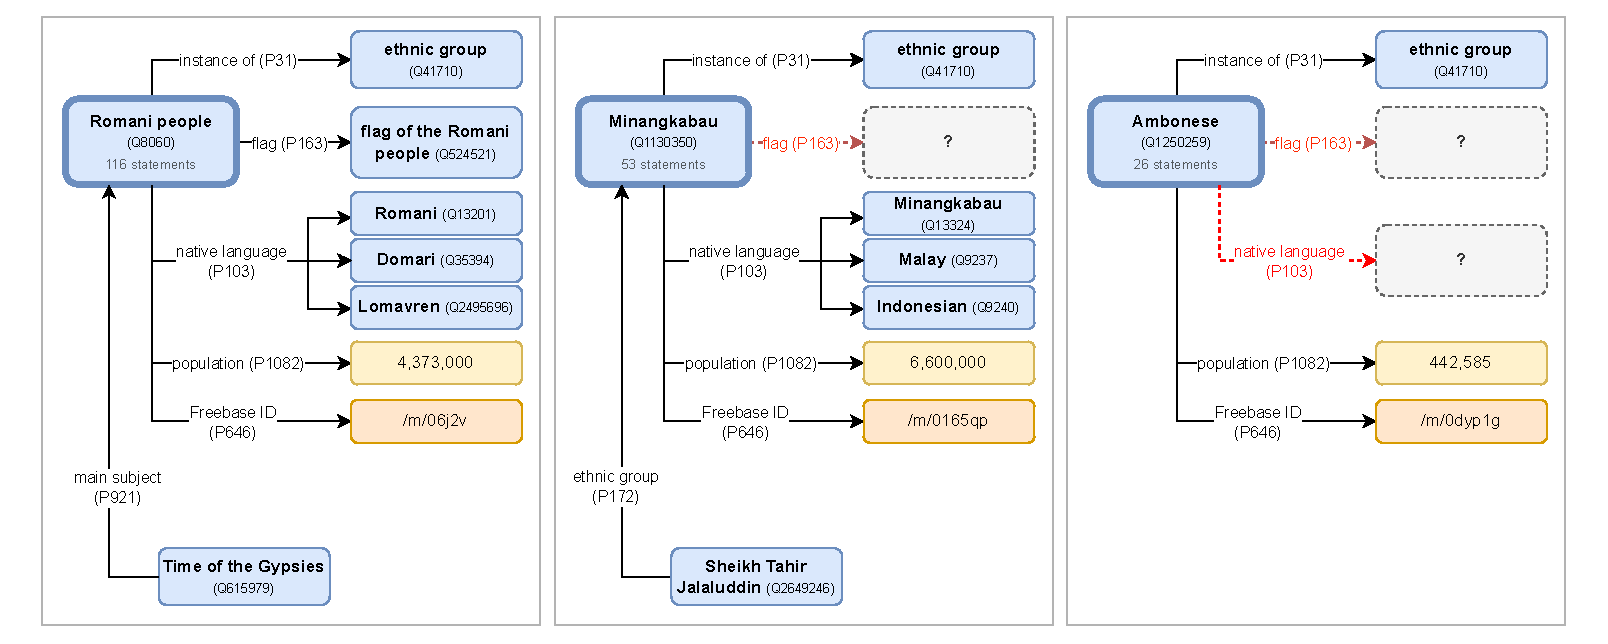
\includegraphics[width=1\textwidth]{Introduction - Wikidata 2}}%
    \caption{Data on Wikidata about the Romani people, the Minangkabau, and the Ambonese. This figure illustrates how entities of the same class can have variations in their representation, including differences in (i) the properties associated with them, (ii) the data types of property values (e.g., objects vs. literals vs. IDs), (iii) the cardinality of properties (single vs. multiple values), and (iv) the direction of information association (whether entities appear in the subject or object position in RDF triples).} \label{fig:intro-wikidata}
\end{figure}

Wealth is the abundance of valuable possessions or money, or the state of having this abundance~\cite{wealthOed}. In economics, wealth is defined as the current market value of all assets owned by individuals or households, calculated as total assets minus liabilities~\cite{SaezG16}. When considering individual (human) wealth, the most common measure is net worth. For instance, in Indonesia, wealth reporting for public officials is conducted through the \textit{Laporan Harta Kekayaan Penyelenggara Negara} (LHKPN\footnote{State Official Wealth Report, a mandatory annual report that requires government officials to report their assets to Indonesia's Corruption Eradication Commission (KPK)}), which includes components such as immovable assets (e.g., land and buildings), movable assets (e.g., vehicles), securities, cash and cash equivalents, receivables, and liabilities. On the other hand, in knowledge graphs (KGs), wealth can be defined as the amount of information (in terms of properties or links) an entity possesses. Just like the different components of wealth in LHKPN, the wealth of an entity in a KG can be calculated based on different types of properties or links, and with different notion of calculation.

\autoref{fig:intro-wikidata} shows three Wikidata entities of the type ethnic group: the Romani people, the Minangkabau, and the Ambonese, along with some information about them. For example, the entity Romani people includes information such as its class, flag, native languages, population, and associated Freebase ID. We can observe that a type of information can have a single value, such as the property \textit{flag} for each entity, which is exactly one (or zero, if the information does not exist), or multiple value, such as the property \textit{native languange}. Both of these properties have values that are other Wikidata entities. Additionally, there are other types of properties, such as \textit{population}, which has a static numerical value, and \textit{Freebase ID}, which provides a string used to identify the entity in the Freebase database.

While the previous examples focus on information with outgoing links, we can also consider the opposite perspective by examining incoming links. This approach does not directly show the possessions of an entity but rather indicates its popularity by showing how often it is mentioned elsewhere. This is illustrated by the Romani people being mentioned in \textit{Time of the Gypsies} and the Minangkabau being associated with Sheikh Tahir Jalaluddin.

The example in \autoref{fig:intro-wikidata} provides a clear picture of how entities in Wikidata can have different kinds and amounts of information, which may lead to knowledge imbalance. If this issue is left unaddressed, it can be problematic for anyone utilizing open KGs as a data source. Data users may draw invalid inferences and conclusions based on incomplete or imbalanced data, such as the Minangkabau and Ambonese are less important than the Romani. Moreover, if contributors to open KGs cannot identify which entities or classes are lacking information, efforts such as editathons may not be effective, potentially widening the gap between information-rich and information-poor entities. For example, contributors might prioritize enriching the Romani people's data while overlooking gaps in the Minangkabau entry, leaving the \textit{flag} property in the Minangkabau empty despite the well-documented existence of the Marawa flag of Minangkabau.

% Existing approaches often focus on ...., lacking a way of quantifying the amount of information contained in KGs. Our study addresses this gap by proposing a formal model to define the knowledge wealth in the RDF knowledge graph. Additionally, we construct an analytical framework using statistical measures and visualization to give insights about the wealth of a class, the inequality between classes, and imbalance measure of wealth within a class. To evaluate this framework, we conducted several use cases on various classes in Wikidata.

% Our contributions are:
% \begin{enumerate}
%     \item We introduce the 3 notions of quantifying knowledge wealth for knowledge graphs, and show how they can be used to further characterize knowledge wealth in knowledge graphs.
%     \item We implemented the formal and insight model using Python programming language and made it accessible.
%     \item We perform a case study on Wikidata classes, showing how biases can be identified in Wikidata, how different definition of wealth impacts the imbalance level of a class, and how the composisition of wealth based on is.
% \end{enumerate}

% Existing approaches often focus on (...), lacking a way of quantifying the amount of information contained in KGs. Our study addresses this gap by proposing a formal model to define the knowledge wealth in the RDF knowledge graph. Specifically, we focus on three key contributions: (i) introducing three notions of quantifying knowledge wealth for knowledge graphs and demonstrating how they can be used to further characterize knowledge wealth; (ii) implementing the formal and insight model using Python and making it accessible for broader use; and (iii) conducting a case study on Wikidata classes, illustrating how biases can be identified, how different definitions of wealth impact the imbalance level of a class, and how the composition of wealth varies between classes.

Existing approaches often focus on (...), lacking a way of quantifying the amount of information contained in KGs. However, quantification of the amount of information is important to ensure more effective effort in tackling the imbalance and incompleteness issue within KGs. From the previous example, we already see the wealth of an entity from three different views: wealth based on the cardinality of property, wealth based on types of property, and wealth based on the direction of link. In addressing the aforementioned gap, our study proposes a formal model to define the knowledge wealth in the RDF knowledge graph.

Specifically, we focus on three key contributions: \text{(i)} introducing three notions of quantifying knowledge wealth for knowledge graphs and demonstrating how they can be used to further characterize knowledge wealth; \textit{(ii)} implementing the formal and insight model using Python and making it accessible for broader use; and \textit{(iii)} conducting a case study on Wikidata classes, illustrating how biases can be identified, how different definitions of wealth impact the imbalance level of a class, and how the composition of wealth varies between classes.

The remainder of this paper is organized into the following sections: Section 2 reviews related work on data completeness and knowledge gaps in knowledge graphs, highlighting existing methodologies and their limitations; Section 3 introduces the proposed knowledge wealth analytics framework, detailing its formal model, statistical measures, and implementation; Section 4 presents the use cases and evaluation results, demonstrating the framework's effectiveness in identifying knowledge gaps within Wikidata; and Section 5 discusses the broader implications of the findings, potential improvements, and future research directions before concluding the study.

%% can be formal background and literature studies
% \section{Related Work} (Pak FD)

% \paragraph{Data Completeness Profiling} Wisesa et al. (2019) presented ProWD, a framework and web application tool for profiling the completeness of Wikidata. It is used to provide insight on degree of attribute completeness of a class in Wikidata. The visualization provided in the we dashboard is equipped with single, compare, or multidimensional view to help in analyzing the facet at entity or class level.

% \paragraph{Imbalance and Gap in Wikidata}
% - Refo: Gini index

% - Nio: gap property
% Ramadizsa1 et al. (2023) introduced the concept of gap properties that helps to characterize class-level knowledge gaps within knowledge graphs. The framework adapts association rule mining to determine ...

\section{Related Work}

In this section, we present related work in knowledge graph (KG) population, KG completeness, and knowledge gaps. KG population concerns adding more information about entities in a KG, thus enriching the knowledge wealth of such entities. KG completeness deals with ensuring whether sufficient information in a KG is available for the task at hand. Intuitively, when a KG possesses more wealth, it has a better chance of being complete for a given task. Knowledge gaps, on the other hand, focus more on measuring whether knowledge wealth in a KG is accumulated in an imbalanced manner.

\paragraph{KG Population.}
Mihindukulasooriya~\cite{Mihindukulasooriya24} introduced a tool and a method to populate Wikidata with scholarly information from DBLP, particularly co-authors and proceedings.
Furthermore, Mihindukulasooriya et al.~\cite{MihindukulasooriyaTDNCP24} argued that Wikidata offers a sustainable approach to providing structured scholarly data and that they developed an LLM-based method to populate Wikidata with conference metadata from unstructured sources.
They analyzed 105 Semantic Web-related conferences and improved the description of over 6000 Wikidata entities. Bolinches and Garijo~\cite{BolinchesG23} made available in Wikidata links between software and their related articles through their SALTbot tool. In addition to creating a new software item in Wikidata (if not there yet), SALTbot will add properties such as ``main subject software'' and also its inverse, ``described by source article''. These initiatives demonstrate that improving the quantity in Wikidata is crucial and that measuring how such an improvement makes a difference (by computing the wealth difference of the before-and-after state) is, therefore, a great addition to such efforts.

\paragraph{KG Completeness.} Wang and Strong~\cite{WangS96} devised a conceptual framework of data quality, highlighting related aspects such as completeness and the appropriate amount of data. Similarly, Zaveri et al.~\cite{ZaveriRMPLA16} conducted a systematic review of Linked Data (LD) quality dimensions, focusing on aspects like relevancy (R2) and completeness.
Wisesa et al.~\cite{WisesaDKNR19} contributed by developing a tool to profile attribute completeness in Wikidata, aligning with initiatives aimed at assessing data quality. Issa et al.~\cite{IssaAHCDZ21} provided a comprehensive review of knowledge graph completeness research, identifying seven distinct types of completeness.
Additionally, Luthfi et al.~\cite{LuthfiDA22} introduced a SHACL-based method to profile completeness in knowledge graphs, further expanding the methodologies available for evaluating data quality. In~\cite{XueZ23}, Xue and Zou surveyed related work on KG quality management. They discovered that most of the work focused on accuracy and completeness. In contrast, no mention was made about the work in KG gaps/imbalances.

\paragraph{Knowledge Gaps.} Ramadhana et al.~\cite{RamadhanaDPNRA20} designed a tool for analyzing knowledge imbalances. The tool featured property quantification for classes and Gini index analysis. Nevertheless, the tool focused only on Wikidata and did not offer fine-grained measures for wealth and imbalances.
Ramadizsa et al.~\cite{RamadizsaDNR23} introduced the concept of gap properties that helps to characterize class-level knowledge gaps within knowledge graphs. The framework adapts association rule mining and empirically analyzes property gaps among various Wikidata classes.
Our work complements both of the work with more general yet more detailed wealth analysis over KGs, including Wikidata. Furthermore, in~\cite{AbianMS22}, Abi{\'{a}}n et al.\ examined gaps in Wikidata content, analyzing edit metrics (contributions to Wikidata) in relation to corresponding Wikipedia pageviews (user needs). Their findings suggest that gaps in gender and recency are not driven by internal factors within Wikidata. However, gaps related to socio-economic factors may be partially endogenous to Wikidata.

%% can be formalization
\section{Knowledge Wealth Framework}

% - RDF model, triples
% - definition of wealth berdasarkan property (kardinalitas, tipe properti, arah properti)
% - insight model

In this section, we define the formal framework for measuring knowledge wealth in knowledge graphs (KGs). We start by introducing the underlying data model based on RDF structure and how entities are represented through triples. Then, we formalize different notions of knowledge wealth using property-based metrics. Lastly, we present an insight model that supports both quantitative analysis and qualitative interpretation of wealth distributions across entity classes.

\subsection{Wealth Formal Model}
Knowledge graphs follow Resource Description Framework (RDF) as a means of data organization. Data is stored in the form of triple \((s, p, o)\); a combination of a subject \(s\), a predicate \(p\), and an object \(o\) which can be visualized as nodes and directed-arc diagrams. For example, the statement "William Shakespeare's notable work is Romeo and Juliet" is mapped to the triple (\textit{WilliamShakespeare}, \textit{notableWork}, \textit{RomeoAndJuliet}).

There are 3 kind of nodes: IRIs, literals, and blank nodes. A triple is in the form of \((s, p, o) \in G) \cap (I \cup B) \times I \times (I \cup B \cup L) \) where \(I\) is the node with type IRIs, \(B\) is the node with type of blank node, and \(L\) is the node with type of literals.

\subsubsection{Class}
In this study, we re-use the class model defined by Ramadizsa et al. (2023). A class is a group of entities that are the subject of the study. \textit{Human}, \textit{film}, and \textit{taxon} are some examples of class. In general, entity \(s\) is an instance of class \(C\) is expressed by the triple (\(s\), \textit{instanceOf}, \(C\)). We can get a more narrow class inside the defined class by specifying additional conditions, each consisting of a particular property and value associated with it. Example of such conditions for human class is \textit{gender} with associated value \textit{male}, while example for a country would be \textit{continent} with value \textit{Asia}. For instance, the class of human with gender male that lived during English Renaissance is queried using
\[
    (?s, \{(?s, instanceOf, Human), (?s, gender, male), (?s, timePeriod, EnglishRenaissance)\})
\]

\subsubsection{Entity-Level Wealth: Knowledge Wealth Type and Definition}

\begin{figure}
     \centering
     \begin{subfigure}[b]{0.3\textwidth}
         \centering
         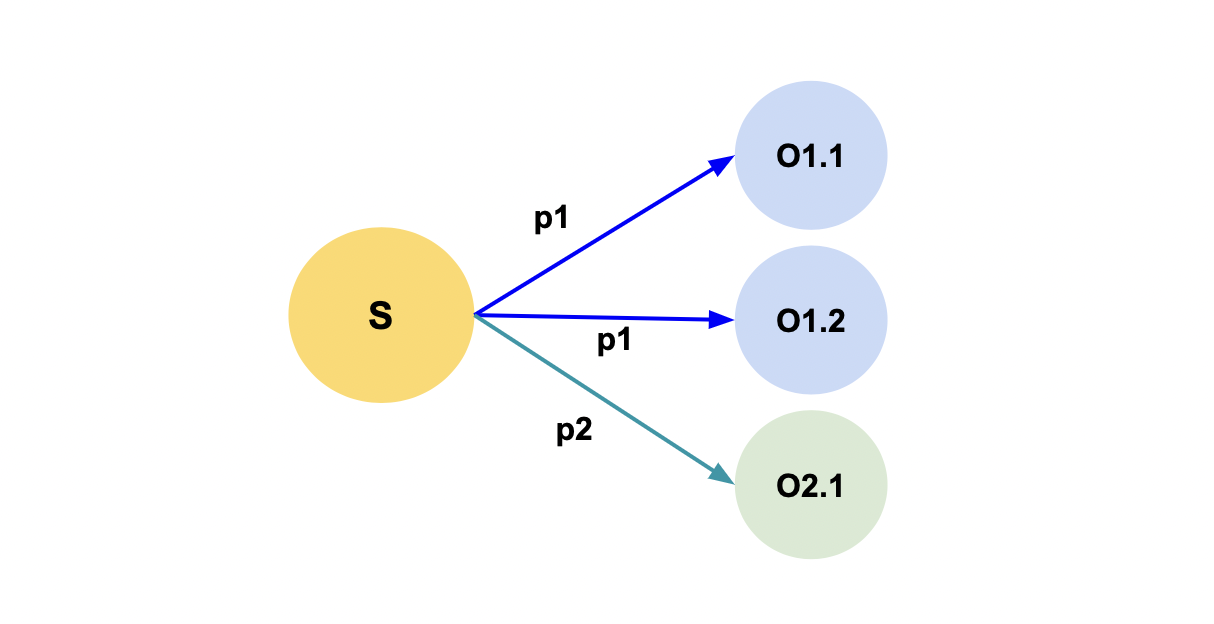
\includegraphics[scale=.3]{Wealth Type 1}
         \caption{Illustration of bag of properties and set of properties}
         \label{fig:wealth-type1}
     \end{subfigure}
     \hfill
     \begin{subfigure}[b]{0.3\textwidth}
         \centering
         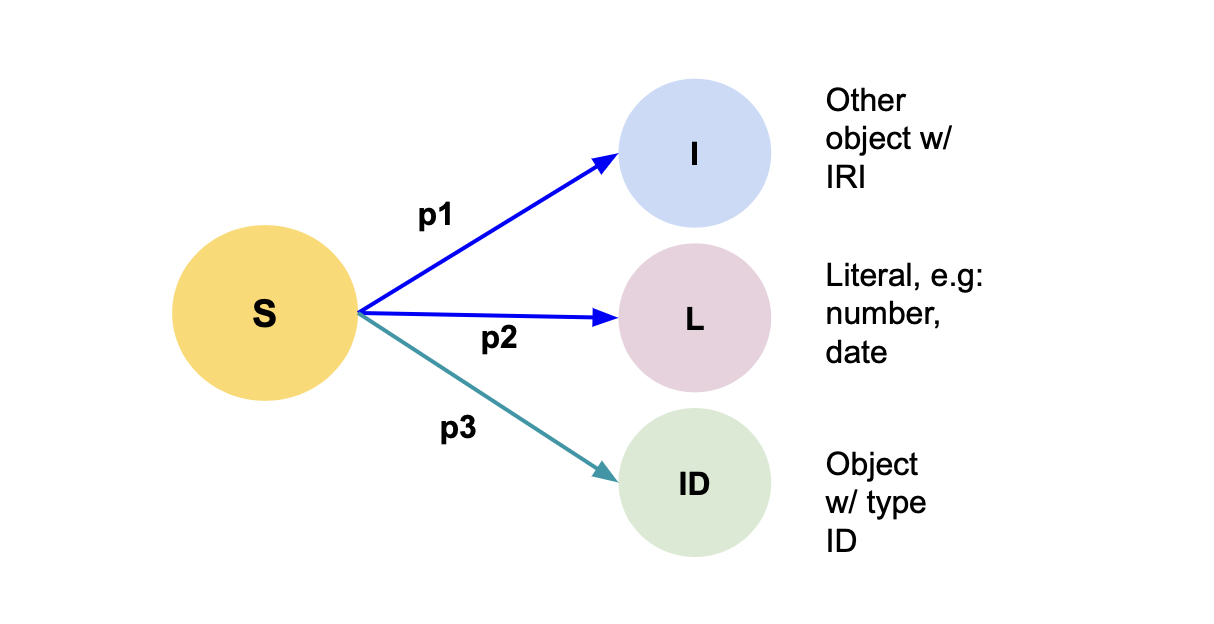
\includegraphics[scale=.3]{Wealth Type 2}
         \caption{Illustration of 3 types of property: object, literal, ID}
         \label{fig:wealth-type2}
     \end{subfigure}
     \hfill
     \begin{subfigure}[b]{0.3\textwidth}
         \centering
         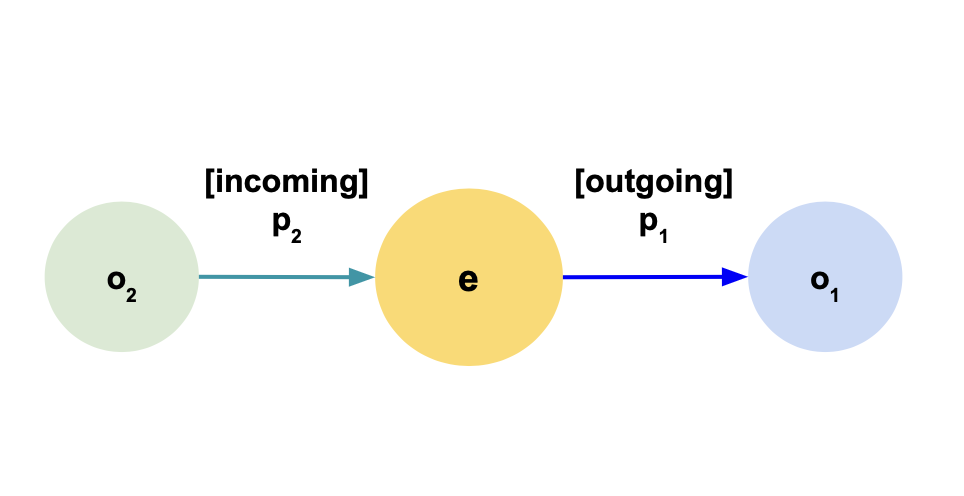
\includegraphics[scale=.3]{Wealth Type 3}
         \caption{Illustration of incoming link vs. outgoing link}
         \label{fig:wealth-type3}
     \end{subfigure}
     \caption{Three simple graphs}
     \label{fig:three graphs}
\end{figure}

Let \(s\) be any entity in a knowledge graph \(G\). We quantify the wealth of entity \(s\) in \(G\) as the amount of information about \(s\) available in \(G\). Thus, the knowledge wealth of an entity is defined by the number of properties associated/linked to it. For example, the wealth of William Shakespeare (Q692) in Wikidata counts all triples describing Q692 in Wikidata, including those detailing his family, occupation, image, and so on.

There are several notion on how to calculate the knowledge wealth of an entity: (1) wealth based on the (non-)uniqueness of individual property; (2) wealth based on type of property; and (3) wealth based on the direction of the link. The wealth of \(s\) with regard to graph \(G\) for each wealth category is denoted by \(W\), formalized and explained as follows.

\paragraph{Wealth based on the (non-)uniqueness of individual properties}
The first measure of the knowledge wealth of \(s\) is bag of properties---the cardinality of set of all triples that has \(s\) in their subject position. In this definition, the triples \((s, p_1, o_1)\) and \((s, p_1, o_2)\) account for a wealth of 1 each, thus both have a total of 2.
Let \(N_{bag}(s,G)\) be a set that comprises all pair of predicate/property and object \((p,o)\) that is connected to \(s\). Then \(W_{bag}(s, G)\) is the cardinality of \(N_{bag}(s,G)\).
\[
    N_{bag}(s,G) = \{(p, o) | (s, p, o) \in G\}
\]
\[
    W_{bag}(s,G) = |N_{bag}(s)|
\]

Another way of measuring the wealth is by counting the number of distinct properties describing the entity, or set of properties. By this way, we are capturing the variety of information about an entity. In contrast to bag of properties, in set of properties \((s, p_1, o_1)\) and \((s, p_1, o_2)\) would be regarded as the "same" information because of the identical property \(p_1\), thus they only account for a total wealth of 1. Let \(N_{set}(s,G)\) be a set that comprises all predicate/property \(p\) that is connected to \(s\). Then \(W_{set}(s, G)\) is the cardinality of \(N_{set}(s,G)\).
\[
    N_{set}(s, G) = \{p | \exists o, (s, p, o) \in G\}
\]
\[
    W_{set}(s, G) = |N_{set}(s,G)|
\]

By the above definition, the wealth of entity \(s\) in \autoref{fig:wealth-type1} is 3 and 2, using bag of properties and set of properties respectively.

\paragraph{Wealth based on type of property}
Object properties are other entities besides \(s\) that is connected with \(s\) through a property \(p\). Wealth of \(s\) using bag of properties with only considering the object properties is defined as:
\[
    W_{bag, object}(s, G) = |\{(p,o) | ((s, p, o) \in G) \cap (o \in I)\}|
\]
Data properties are non-object properties that is connected with \(s\) through a property \(p\). Wealth of \(s\) using bag of properties with only considering the data properties is defined as:
\[
    W_{bag, data}(s, G) = |\{(p,o) | ((s, p, o) \in G) \cap (o \in L)\}|
\]

An external ID is a special type of string that is used to represent an entity in an external source. In Wikidata, an ID is element of subclass of \textit{Wikidata property for an identifier} (Q19847637). Just like any other property, an ID is connected with \(s\) through a property \(p\). Let  \(C_{ID,G}\) be a set comprising ID property in graph \(G\). Wealth of \(s\) using bag of properties with only considering the ID properties is defined as:
\[
    W_{bag, ID}(s, G) = |\{(p,o) | ((s, p, o) \in G) \cap (o \in L) \cap (o \in C_{ID,G})\}|
\]

\paragraph{Wealth based on the direction of the link}
In outgoing link type of wealth, the properties that are used in the wealth calculation of an entity \(s\) are those obtained from link with outwards direction from that particular entity \(s\); that is where \(s\) appears to be the subject in the set of triples in graph \(G\). All types of wealth defined before use the notion of outgoing link.

In incoming link type of wealth, the properties that are used in the wealth calculation of an entity \(s\) are those obtained from link with inwards direction to that particular entity \(s\); that is where \(s\) appears to be the object in the set of triples in graph \(G\). To illustrate, let \(N_{bag}(s)\) be a set that comprises all pair of object and predicate/property \((o,P)\) that is connected to \(s\) in incoming direction to \(s\) i.e., \(N_{bag}(s)\) = \(\{(o, p) | (o, p, s) \in G\}\). Then the wealth of \(s\) using bag of properties and the view of incoming link is notated as \(W_{bag, incoming}(s, G)\), and equal to the cardinality of \(N_{bag}(s)\).
\[
    N_{bag, incoming}(s, G) = \{(o,p) | (o, p, s) \in G\}
\]
\[
    W_{bag, incoming}(s, G) = |N_{bag, incoming}(s, G)|
\]

Looking at in \autoref{fig:wealth-type3}, the wealth of entity \(s\) is 1 using outgoing link, which is from the triple \((s, p_1, o1)\). Its wealth is also 1 and using incoming link, which comes from the triple \((o2, p_2, s)\).

Each definition above can be used simultaneously. For example, the wealth of entity \(s\) using set of properties, calculating object and data but not ID properties, and using the direction of outgoing link is denoted by \(W_{set, outgoing, (object \cup data) \cap ID^\complement}(s, G) = |N_{set, outgoing, (object \cup data) \cap ID^\complement}(s, G)|\) with \(N_{set, outgoing, (object \cup data) \cap ID^\complement}(s, G) = \{p | \exists o, (s, p, o) \in G, \cap (o \in ((I \cup L) \cap C_{ID,G}^\complement)\}\)

\subsubsection{Class-Level Wealth}
Let \(C\) be a class that consists of \(m\) distinct entities \(s_1\), \(s_2\), ... \(s_m\) in graph \(G\). The wealth of \(C\) can be be quantified using its constituent entities. It can be described by several measures, such as entity count, mean and median of its entities' wealth, and percentile of its entities's wealth. To illustrate, let a class \(C\) consists of 4 entities  \(s_1\), \(s_2\), \(s_3\), and \(s_4\) from \autoref{fig:wealth-weighted}. We may say class \(C\) has a total wealth of 4 when we look from count of entities.
\subsection{Insight Model}

\paragraph{Exploratory Data Analysis (EDA): Descriptive Statistics Measures.} Descriptive statistics is concerned with the description and summarization of data. It is a summary of a dataset that helps to describe features of data quantitatively (Ross, 2019). To have a general view of wealth distribution of a class, we use the following measures:
\begin{itemize}
  \item measures of central tendency: mean, median, mode
  \item measures of frequency: count, cumulative frequency/percentage
  \item measures of position: quartile, percentile
  \item measures of dispersion: minimum, maximum, range, interquartile range, standard deviation, coefficient of variation, kurtosis
  \item measures of symmetry: skewness
\end{itemize}


\paragraph{Gini Coefficient}
Gini coefficient is a metric used to measure the economic wealth gaps between countries. A study by Akbar (2020) utilized the Gini coefficient to measure the level of knowledge imbalance in knowledge graphs, particularly Wikidata classes. To calculate the imbalance level of a Wikidata class using Gini coefficient, the researcher started by calculating the number of properties of each entity of that particular class and storing them in an array. The array will then be sorted in descending order, from the smallest to the largest i.e., \(y_{i} \geq y_{i+1} \forall i \in \{1, 2, ..., n\}\). The Gini coefficient will be calculated from the sorted array using the Gini coefficient formula below.

\[G = 1 - \frac{1}{n^{2}\mu} \sum_{i=1}^{n} \sum_{j=1}^{n} Min(y_{i}, y_{j})\]
\[G = 1 + \frac{1}{n} - \frac{1}{n^{2}\mu} - (y_{1} + 2y_{2} + ... + ny_{n})\]

In economics context, \(n\) is the size of population of a country, $\mu$ is the average income, and \(y\) is an array containing data of each country's income. However, in the context of knowledge graph, \(n\) is the number of entities in the class, $\mu$ is the average knowledge wealth of the entities, and \(y\) is an array containing data of each entity's wealth, sorted in descending order.

For example, let's say we have a class that consists of 10 entities. After counting the number of properties of each entities (using the notion of bag of properties for wealth) and sorting them in descending order, we will have an array of \(y = [10,8,8,7,4,2,2,1,1,1]\). The length of the array is \(n = 10\) and the average wealth is \(\mu = 4.4\). Then, apply the Gini coefficient formula and we get \(G = 1 + \frac{1}{10} - \frac{2}{10^{2}\times4.4}(1\times10 + 2\times8 + ... + 10\times1) = 0.414\)

For another another example, let's say we have another array of 10 entities \(z = [10, 9, 9, 9, 9, 9, 9, 9, 9, 5]\). By applying the same formula to z, we get a Gini coefficient value of \(0.052\).

The Gini coefficient has a value between \(0\) and \(1\). The higher the coefficient value, the greater the imbalance level. The value of 0 is achieved when all observed entities have the same amount of wealth. The value of 1 occurs when all income is owned solely by one entity and this phenomenon expresses full inequality.


\paragraph{Lorenz Curve} Lorenz curve is a graphical representation of wealth inequality (The Lorenz Curve: What It Tells You About Economic Inequality, 2022). It shows how the wealth is cumulatively distributed, with data points sorted from the poorest to the richest. \textit{(Here, give the example of Lorenz Curve)}. In Lorenz curve, the horizontal axis represents the fraction of the population, and the vertical axis represents the cumulative wealth. Therefore, if the point (\textit{x}, \textit{y}) = (30, 15) lies on the curve, then we can interpret that the bottom 30\% of the population account for 15\% of the total wealth in that population. The Lorenz curve is usually drawn along with a straight diagonal line with a slope of 1. This straight line represents perfect equality in wealth distribution, i.e., each individual in the observed population has equal wealth. The Lorenz curve itself is drawn below the straight line. The ratio of the area between the Lorenz curve and the straight line of perfect equality to the triangular area below the straight line, is the Gini coefficient.

\subsection{Sample Application of Formal and Insight Model}

\begin{figure}[!htbp]
    \centering
    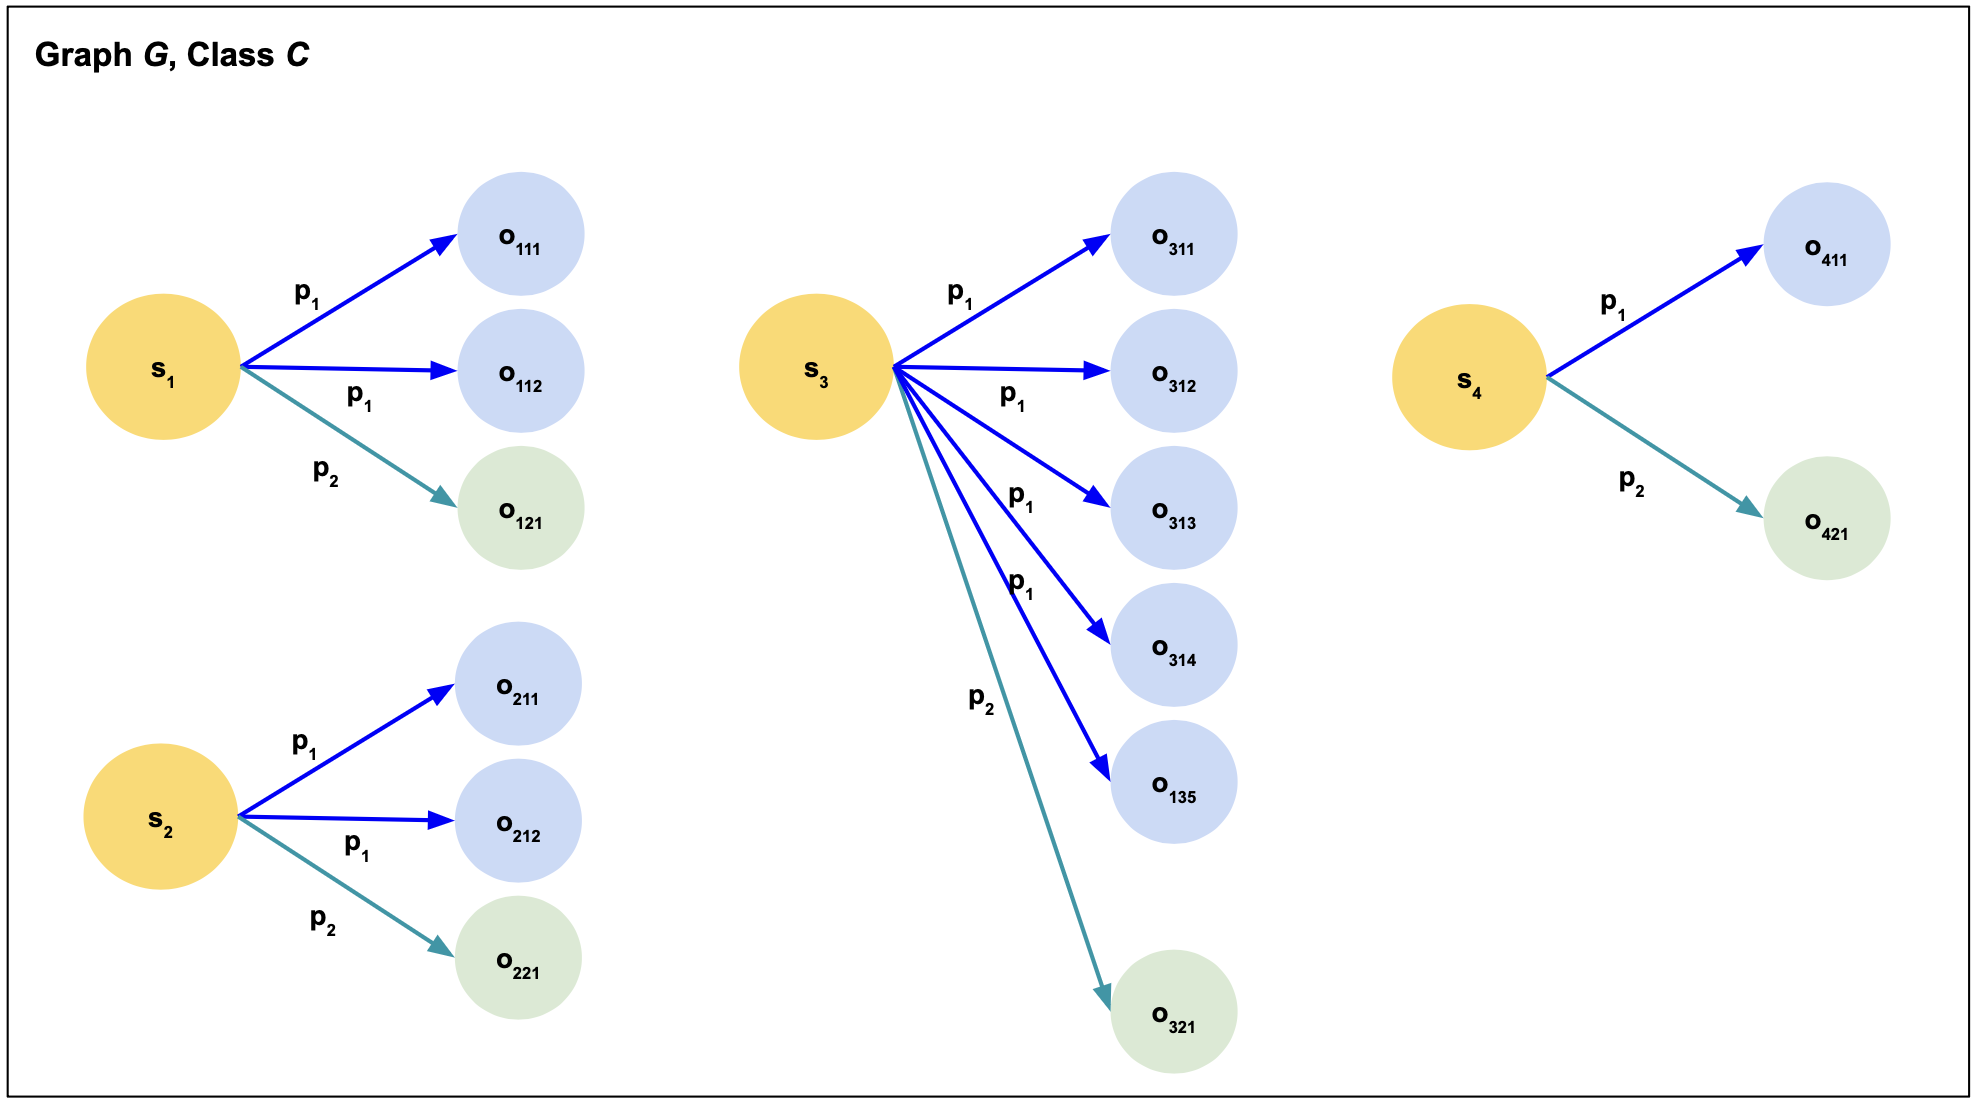
\includegraphics[scale=.4]{Wealth Weighted}
    \caption{Sample knowledge graph \(G\) that contains class \(C\) with 4 entities} \label{fig:wealth-weighted}
\end{figure}

We provide small case in \autoref{fig:wealth-weighted} to illustrate how both models can be applied in quantifying knowledge wealth. In this example, we will focus on the notion using bag of properties with outgoing direction of link to quantify the wealth.

A graph \(G\) has a class \(C\), which consists of four entities \(s_1\), \(s_2\), \(s_3\), and \(s_4\). Each entity has two distinct properties \(p_1\) and \(p_2\). For example, entity \(s_1\) is linked by property \(p_1\) to objects \(o_{111}\) and \(o_{112}\), and by property \(p_2\) to object \(o_{121}\). Using the bag of properties and outgoing link direction, the wealth of entity \(s_1\) is 3 (2 accounted for by \(p_1\) and 1 by \(p_2\)). Similarly, the wealth of entities \(s_2\), \(s_3\), and \(s_4\) is 3, 6, and 2, respectively. \autoref{tab:sample statistical summary} provides a statistical summary describing the wealth of class \(C\). Entities in class \(C\) have a mean wealth of 3.5, a median wealth of 3, a mode wealth of 3, a minimum wealth of 2, and a maximum wealth of 6. Based on each individual entity's wealth, the imbalance measure of class \(C\) is quantified using the Gini coefficient, which has a value of 0.21.

\begin{center}
    \small
    \begin{threeparttable}
    \caption{Statistical Summary of Wealth of Class \(C\)}
    \label{tab:sample statistical summary}
    \begin{tabular}{c | c c c c c c c} 
    
    \toprule
        Measure & Entity Count & Mean & Median & Mode & Minimum & Maximum & Gini \\ [0.5ex] 
    \midrule
        Value & 4 & 3.5 & 3 & 3 & 2 & 6 & 0.21 \\
        [0.5ex]
    \bottomrule
    \end{tabular}
    \begin{tablenotes}
        \footnotesize
        \item{This table shows some statistical measures to quantify the wealth of class \(C\).}
    \end{tablenotes}
    \end{threeparttable}
\end{center}

In addition to the Gini coefficient, the Lorenz curve for the wealth of entities in class \(C\) is shown in \autoref{fig:sample-lorenz}. This figure illustrates that the wealth distribution within class \(C\) is very close to the diagonal line of perfect equality, which aligns with the small Gini coefficient value of 0.21.

\begin{figure}[!htbp]
    \centering
    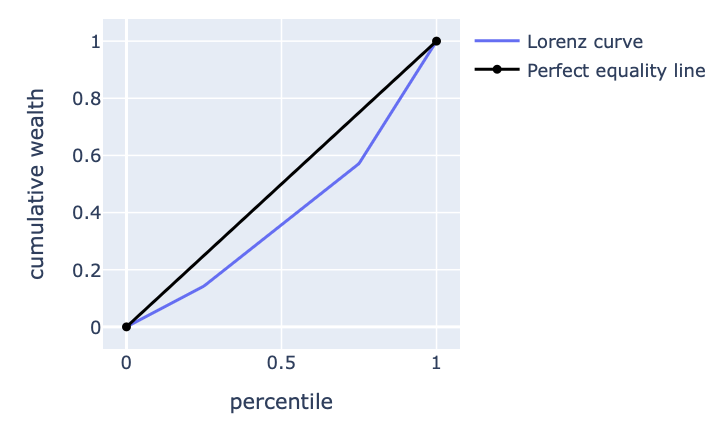
\includegraphics[scale=0.8]{Sample Lorenz Curve}
    \caption{Lorenz curve of class \(C\)} \label{fig:sample-lorenz}
\end{figure}
\subsection{Python-Based Model Implementation}

Our study provides a Python-based implementation library for both the formal model and the insight model. The library incorporates the three notions of knowledge wealth discussed in \autoref{wealth-formal-model}, as well as the insight model outlined in \autoref{insight-model}. While the model is platform-agnostic, i.e., it can be applied to any KG, we focus its implementation on Wikidata for demonstrating its use cases. Wikidata is specifically chosen because of the availability of Wikidata Query Service which  facilitates structured queries over its data.

The notions of wealth are implemented at the query level, meaning that the filters and aggregations based on each wealth definition are directly embedded in SPARQL queries. The flow begins with defining class filters to specify the entities of interest. Next, SPARQL querying is performed using Wikidata Query Service to retrieve RDF triples matching the specified criteria and aggregate them according to the selected notion of wealth. The extracted data is then structured into pandas DataFrames, enabling further analysis through the insight model using Python libraries.

In our implementation, we only consider direct properties and exclude blank nodes to reduce complexity and maintain data quality. The complete flow of the formal model and insight model usage is illustrated in \autoref{fig:model-implementation}.

\begin{figure}[!htbp]
    \centering
    % 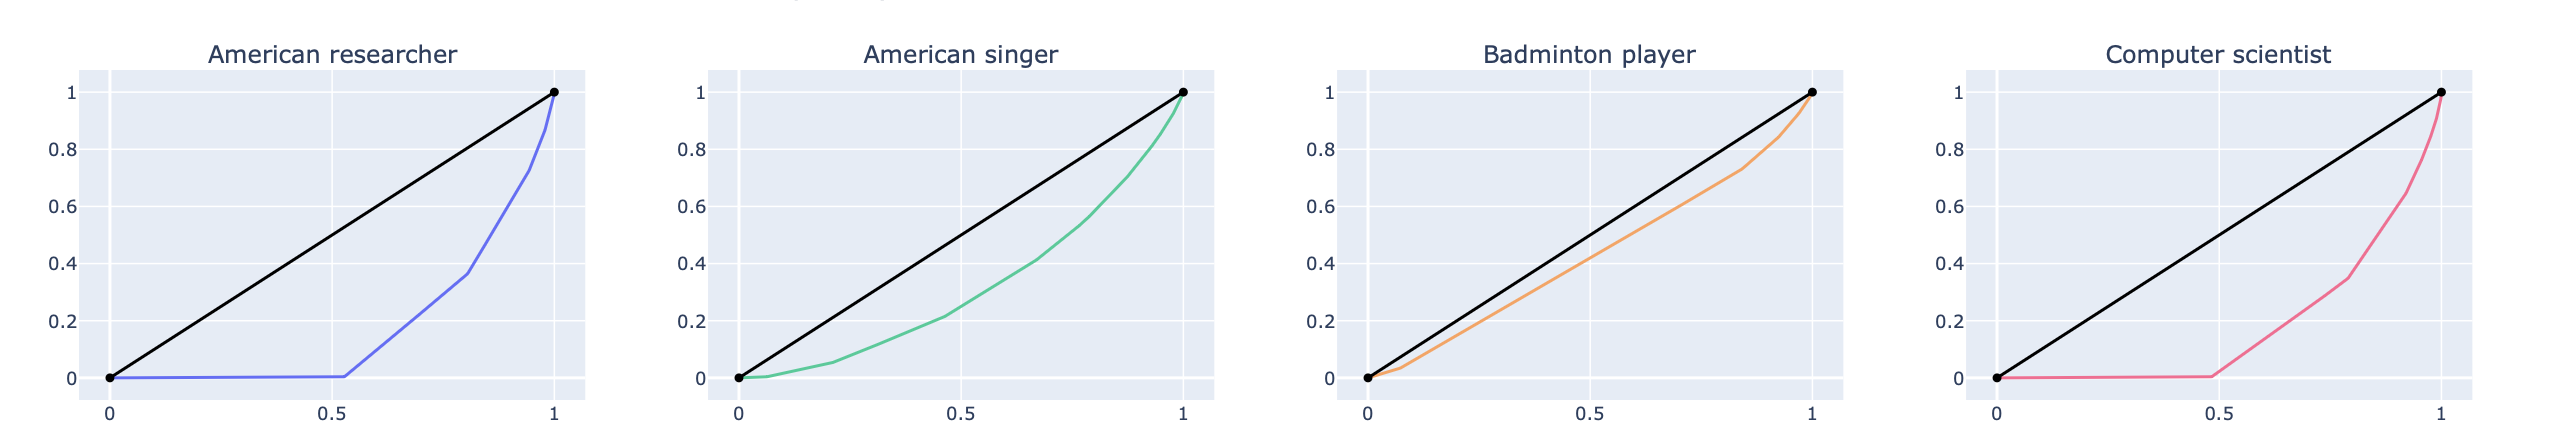
\includegraphics[scale=.5]{Gini - Pure Literal}
    \makebox[\textwidth][c]{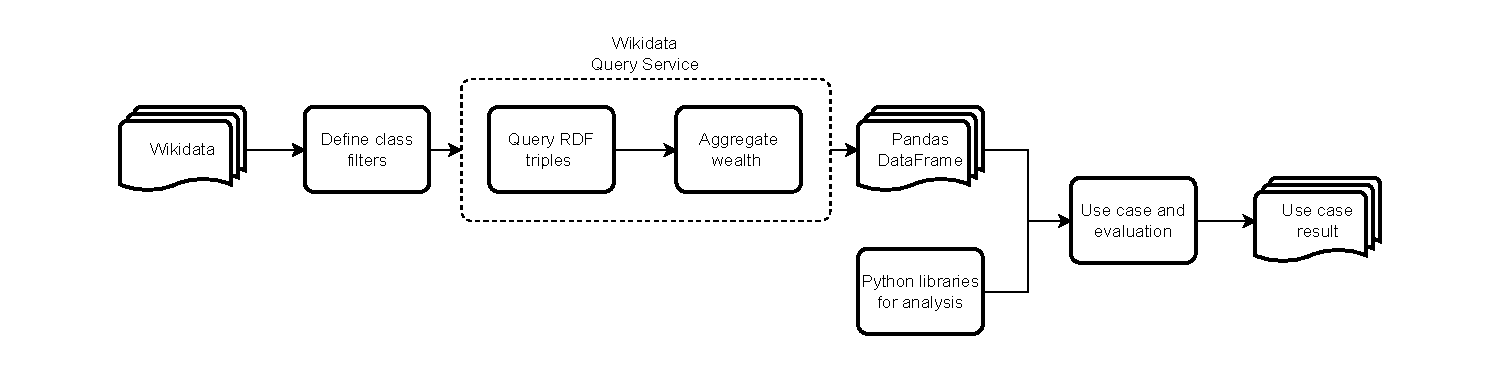
\includegraphics[width=1\textwidth]{Model Implementation.pdf}}%
    \caption{Model implementation and evaluation flow using Python Jupyter Notebook} \label{fig:model-implementation}
\end{figure}

%% application of formal model on WD
\section{Use Cases and Evaluation}

This section will discuss use cases and evaluation of the research. The data used were taken from Wikidata and retrieved using Wikidata Query Service on March 2nd 2025.

% to be added:
% - data di-retrive kapan: [input date]
% - only consider truthy/direct property
% - cara akses data dari Wikidata, flow pemrosesan data (dengan diagram)

% \subsection{Bias in Wikidata}
\subsection{Group-Level Gap in Representation in Wikidata}

In this subchapter, analysis is conducted to see whether any particular entity group in Wikidata is underrepresented compared to others. There are 2 analysis done: gender-based gap and regional gap.


\paragraph{Gender Bias in Wikidata}
Gender bias analysis in Wikidata will be performed on 10 Wikidata classes: computer scientist, American singer, American actress/actor, badminton player, businessperson, lawyer, American politician, American writer, American researcher, and American journalist.

To analyze the bias, the first aspect that will be considered is the proportion of each gender in every class. We assume that there are equal numbers of males and females in real-world and this will be the basis to determine if there is any bias in the data. Pearson's chi-square test (goodness-of-fit) is then performed to test the null and alternative hypotheses with significance level of \(\alpha=5\%\) as follows:

\(H_0\): The proportions of males and females in a particular class are equal to the real-world proportion

\(H_1\): The proportions of males and females in a particular class are not equal to the real-world proportion

From \autoref{tab:gender - entity count}, we can see that there are more male entities than female entities in all of the classes. In terms of entity count, the gender gaps in some classes such as American singer, American actress/actor, badminton player, and American writer, are slim. The gender gaps in some other classes are huge, and it can be observed in the classes of computer scientist, businessperson, lawyer, American politician, journalist, and researcher. This phenomenon can also be easily identified through visualization, as exhibited in \autoref{fig:bias histogram-computer scientist}, where the histogram of the female subclass is much smaller compared to the male. Looking at the chi-square test result, as p-value is well below the chosen significance level, the null hypothesis is rejected in all classes. Hence, we consider the difference of entity count to be significant and conclude that the proportions of males and females in each Wikidata class are not the same as the assumed real-world proportion of 50\%-50\%.

However, it is arguable that, for some classes, the gap in entity count between both genders is expected because, in reality, there are more men than women in the workforce, especially in particular fields such as engineering. As a consequence, it is not reasonable if we expect to have an equal number of males and females entities in Wikidata. Therefore, entity count may not be a good measure of bias because of the nature of the data itself. To address this, we need to evaluate other metrics which can quantify the bias on entity-level.

\begin{center}
\small
\begin{threeparttable}
\caption{Entity Count of 10 Wikidata Classes per Gender Category}
\label{tab:gender - entity count}
\begin{tabular}{c | c c c c c c c} 

\toprule
    Class Name & Entity & Male & Female & \%Male & \%Female & $\chi^2$ & p-value \\ [0.5ex] 

\midrule
    American actress/actor & 38087 & 21451 & 16636 & 0.56 & 0.44 & 608.72 & 2.13e-134 \\
    American journalist & 17740 & 12223 & 5517 & 0.69 & 0.31 & 2534.97 & 0.0 \\
    American politician & 92901 & 83007 & 9894 & 0.89 & 0.11 & 57539.86 & 0.0 \\
    American researcher & 4867 & 3387 & 1480 & 0.70 & 0.30 & 747.21 & 1.63e-164 \\
    American singer & 15712 & 9027 & 6685 & 0.57 & 0.43 & 349.09 & 6.67e-78 \\
    American writer & 32573 & 19113 & 13460 & 0.59 & 0.41 & 981.07 & 2.34e-215 \\
    Computer scientist & 17914 & 15229 & 2685 & 0.85 & 0.15 & 8783.74 & 0.0 \\
    Badminton player & 25283 & 13377 & 11906 & 0.53 & 0.47 & 85.58 & 2.22e-20 \\
    Businessperson & 74538 & 66706 & 7832 & 0.89 & 0.11 & 46501.76 & 0.0 \\
    Lawyer & 91348 & 80639 & 10709 & 0.88 & 0.12 & 53533.79 & 0.0 \\ [1ex]
\bottomrule

\end{tabular}
\begin{tablenotes}
    \footnotesize
    \item{This table shows the entity count of 10 Wikidata classes per Gender Category. Chi-square test result shows the significance of difference between the entity count of the two genders male and female.}
\end{tablenotes}

\end{threeparttable}
\end{center}

The next metrics to be considered are the measures of central tendency and dispersion to see where the wealth distribution is concentrated and how the data spread.

From \autoref{tab:gender - central tendency}, female entities generally have lower values of measure of central tendency (mean, median, mode). These characteristics can also be observed from the histogram in \autoref{fig:bias histogram-computer scientist}: female histograms’ peak and dense area are located on the left of the male’s. The range of property count of females is generally also lower than males. However, there are some classes in which the richest entity is a female. An example for this is the class of American Singer, which is shown by \autoref{fig:bias histogram-american singer}. Though the value of mean, median, and mode of count of properties are lower for female compared to male, the richest entity on that class is a female entity Madonna (Q1744) with bag of property count of 687, with a significant difference with Michael Jackson (Q2831) with bag of property count of 574. We also observed positive values of skewness (skewness > 0) and high kurtosis values (kurtosis > 3) in all classes, denoting the wealth distribution is right skewed and leptokurtic.

\begin{center}
\small
\begin{threeparttable}
\caption{Measures of Central Tendency of 10 Wikidata Classes per Gender Category}
\label{tab:gender - central tendency}
\begin{tabular}{c | c c c} 

\toprule
    Class Name & \CellWithForceBreak{Mean \\ (o/m/f)} & \CellWithForceBreak{Median \\ (o/m/f)} & \CellWithForceBreak{Mode \\ (o/m/f)} \\ [0.5ex] 
\midrule
    American actress/actor & 38.96/39.85/37.80 & 29.00/30.00/28.00 & 19/19/22 \\
    American journalist & 30.71/32.44/26.89 & 23.00/25.00/20.00 & 14/14/14 \\
    American politician & 19.22/19.33/18.25 & 15.00/15.00/15.00 & 13/9/13 \\
    American researcher & 23.97/25.00/21.63 & 20.00/21.00/18.00 & 12/12/12 \\
    American singer & 42.78/42.99/42.51 & 31.00/33.00/30.00 & 18/24/15 \\
    American writer & 38.86/42.76/33.33 & 30.00/33.00/26.00 & 19/22/19 \\
    Computer scientist & 24.16/24.50/22.28 & 19.00/19.00/18.00 & 8/8/8 \\
    Badminton player & 21.50/21.25/21.78 & 16.00/16.00/16.00 & 13/13/13 \\
    Businessperson & 16.91/16.83/17.61 & 13.00/13.00/13.00 & 10/10/9 \\
    Lawyer & 22.44/22.98/18.37 & 19.00/19.00/15.00 & 16/16/12 \\
    [1ex]
\bottomrule
\end{tabular}
\begin{tablenotes}
    \footnotesize
    \item{This table shows the measures of central tendency of 10 Wikidata classes per gender category. Each measure will have 3 values: o (overall), m (male), and f (female).}
\end{tablenotes}
\end{threeparttable}
\end{center}


\begin{center}
\small
\begin{threeparttable}
\caption{Measures of Dispersion and Symmetry of 10 Wikidata Classes per Gender Category}
\label{tab:gender - dispersion and symmetry}
\begin{tabular}{c | c c c c c} 

\toprule
    Class Name & \CellWithForceBreak{Min \\ (o/m/f)} & \CellWithForceBreak{Max \\ (o/m/f)} & \CellWithForceBreak{Std. Deviation \\ (o/m/f)} & \CellWithForceBreak{Skewness \\ (o/m/f)} & \CellWithForceBreak{Kurtosis \\ (o/m/f)} \\ [0.5ex] 
\midrule
    American actress/actor & 4/4/4 & 687/574/687 & 33.89/32.75/35.28 & 4.23/3.54/4.94 & 30.74/21.59/39.53 \\
    American journalist & 4/5/4 & 402/402/353 & 26.84/28.14/23.23 & 4.21/4.18/4.15 & 30.73/30.18/29.38 \\
    American politician & 4/4/4 & 476/476/328 & 14.77/14.77/14.75 & 6.53/6.55/6.40 & 97.36/100.39/72.68 \\
    American researcher & 4/4/4 & 222/222/171 & 16.89/18.19/13.17 & 3.86/3.79/3.45 & 25.67/23.50/26.78 \\
    American singer & 4/4/4 & 687/574/687 & 39.35/35.33/44.21 & 4.09/3.16/4.61 & 29.38/18.24/33.19 \\
    American writer & 4/4/4 & 476/476/425 & 34.12/37.19/28.30 & 3.56/3.29/4.05 & 20.51/17.35/27.82 \\
    Computer scientist & 3/3/3 & 441/441/168 & 19.53/20.18/15.24 & 3.41/3.45/2.20 & 27.66/27.80/9.33 \\
    Badminton player & 4/9/4 & 360/238/360 & 16.09/15.28/16.96 & 4.23/3.89/4.48 & 30.85/22.98/35.97 \\
    Businessperson & 3/3/3 & 574/574/429 & 14.65/14.01/19.27 & 7.73/7.37/8.15 & 130.49/128.49/108.21 \\
    Lawyer & 3/3/3 & 550/550/328 & 16.61/16.91/13.47 & 5.56/5.59/5.23 & 76.02/76.31/64.39 \\[1ex]
\bottomrule
\end{tabular}
\begin{tablenotes}
    \footnotesize
    \item{This table shows the measures of dispersion and symmetry of 10 Wikidata classes per gender category. Each measure will have 3 values: o (overall), m (male), and f (female).}
\end{tablenotes}
\end{threeparttable}
\end{center}

\begin{figure}[htp]
\centering 
\subfloat[Histogram and Marginal Distribution Plot of Wealth for Class Computer Scientist\label{fig:bias histogram-computer scientist}]{%
  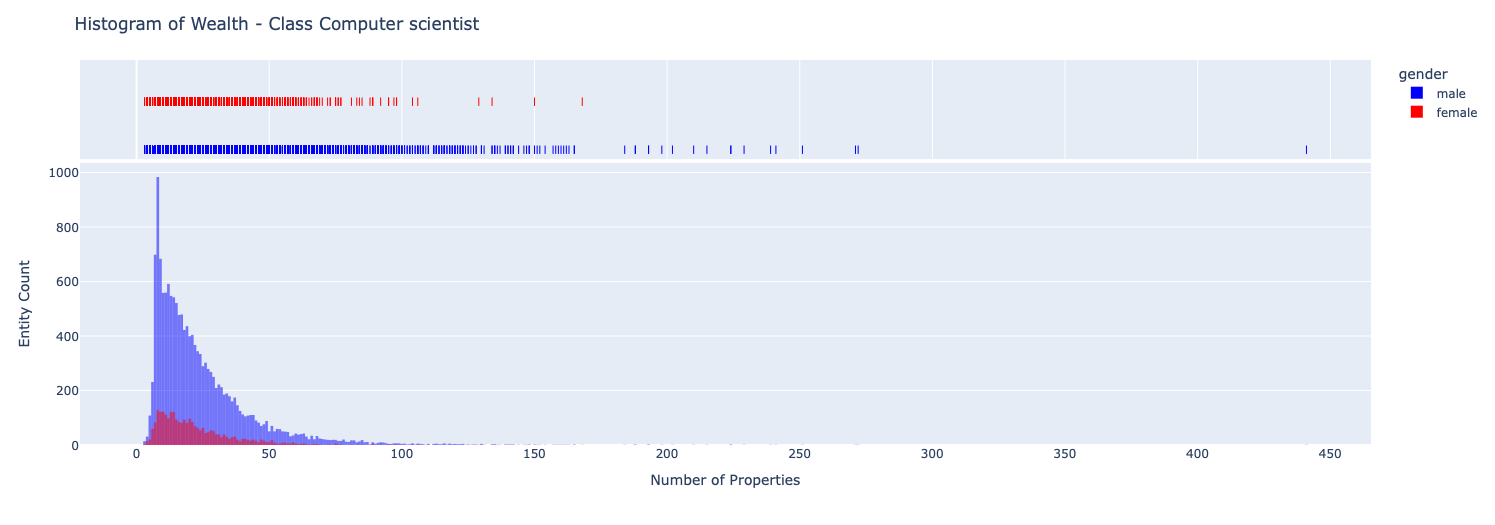
\includegraphics[clip,width=1.0\columnwidth]{Histogram of Wealth - Computer Scientist}%
}

\subfloat[Histogram and Marginal Distribution Plot of Wealth for Class American Singer\label{fig:bias histogram-american singer}]{%
  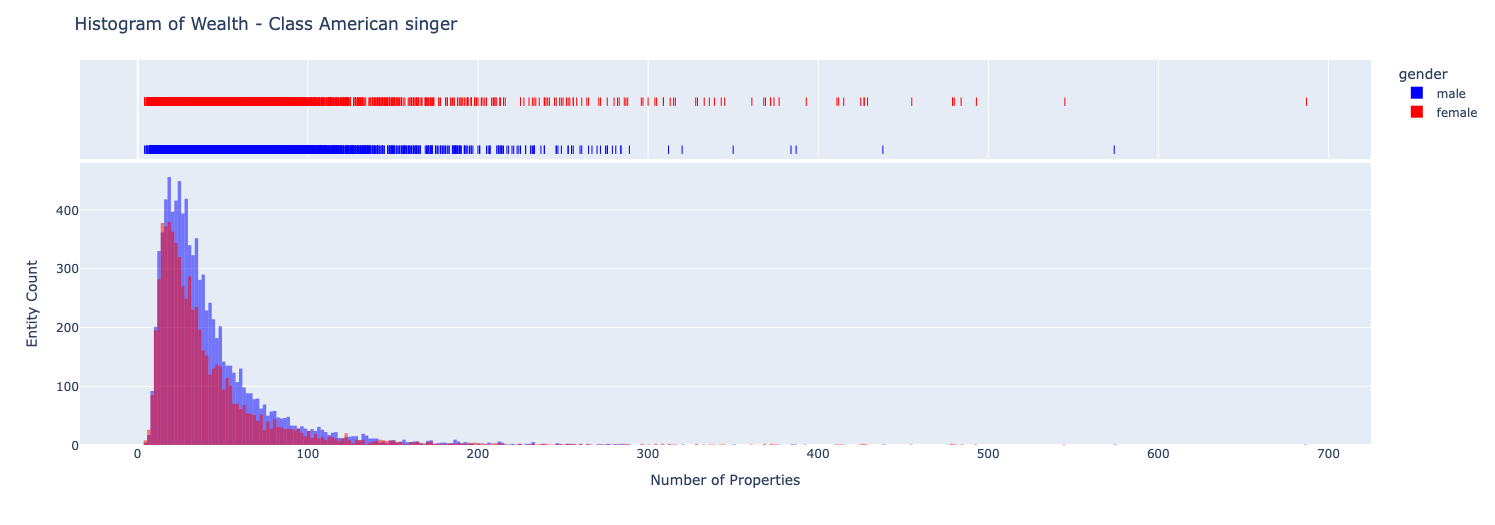
\includegraphics[clip,width=1.0\columnwidth]{Histogram of Wealth - American Singer}%
}

\caption{Histogram of wealth} \label{fig:Histogram of Wealth}

\end{figure}

At a glance we saw female classes are poorer compared to the male classes. To test this, we will use t-test and Welch's test. First, we performed F-test to check if the male and female classes have equal variance. The result of F-test is then used to determine the appropiate test to be used in each class. Those with equal variance will use t-test; otherwise Welch's test is used. Then, we performed the tests to verify the null and alternative hypotheses with significance level of \(\alpha=5\%\) as follows:

\(H_0\): The means of wealth of males and females in a particular class are equal

\(H_1\): The means of wealth of males and females in a particular class are not equal

\begin{center}
\small
\begin{threeparttable}
\caption{F-Test, T-Test, and Welch's Test Result of 10 Wikidata Classes}
\label{tab:gender - mean test}
\begin{tabular}{c | c c c c c c} 

\toprule
    Class Name & \CellWithForceBreak{F-Test \\ statistic} & \CellWithForceBreak{F-Test \\ p-value} & \CellWithForceBreak{T-Test \\ statistic} & \CellWithForceBreak{T-Test \\ p-value} & \CellWithForceBreak{Welch's Test \\ statistic} & \CellWithForceBreak{Welch's \\ p-value} \\ [0.5ex] 

\midrule
    American actress/actor & 0.86 & 0.00 & 5.85 & 4.97e-09 & 5.80 & 6.89e-09\\
    American journalist & 1.47 & 1.00 & 12.80 & 2.45e-37 & 13.75 & 1.01e-42 \\
    American politician & 1.00 & 0.55 & 6.86 & 6.90e-12 & 6.87 & 6.94e-12 \\
    American researcher & 1.91 & 1.00 & 6.43 & 1.35e-10 & 7.28 & 4.15e-13 \\
    American singer & 0.64 & 0.00 & 0.75 & 0.45 & 0.73 & 0.47 \\
    American writer & 1.73 & 1.00 & 24.80 & 1.56e-134 & 25.98 & 2.96e-147 \\
    Computer scientist & 1.75 & 1.00 & 5.43 & 5.57e-08 & 6.60 & 4.61e-11 \\
    Badminton player & 0.81 & 0.00 & -2.63 & 8.46e-03 & -2.62 & 8.86e-03 \\
    Businessperson & 0.53 & 0.00 & -4.48 & 7.56e-06 & -3.49 & 4.81e-04 \\
    Lawyer & 1.58 & 1.00 & 27.06 & 1.16e-160 & 32.16 & 8.04e-220 \\
    [1ex]

\bottomrule

\end{tabular}
\begin{tablenotes}
    \footnotesize
    \item{}
\end{tablenotes}
\end{threeparttable}
\end{center}

From the test results in \autoref{tab:gender - mean test}, we rejected the null hypothesis in 9 out of 10 class--American singer being the only exception. 7 out of 9 classes are in favor of male. The other 2 classes, American singer and . We concluded that female classes are more likely to have smaller means than male classes.

Here, a new measure is defined: top \(x\)\% male/female relative to the expectation. The value of expectation of a gender in a class is equal to the percentage of that particular in the class. Top \(x\)\% male relative to expectation is the ratio of percentage of male entities in the top \(x\)\% to the expectation. Similarly, top \(x\)\% female relative to expectation is the ratio of percentage of female entities in the top \(x\)\% to the expectation.

When the shape of distribution of male and female of a class is the same (in other word, the wealth is distributed equivalently to male and female entities), then the value of top \(x\)\% relative to expectation should be 1 for both male and female subclasses. A value higher than 1 indicates domination by that particular gender.

\begin{figure}[htp]
\centering 
\subfloat[Ratio of Class Wealth to Expectation per Cumulative Top Percentage - All Classes Average
\label{fig:test1}]{%
  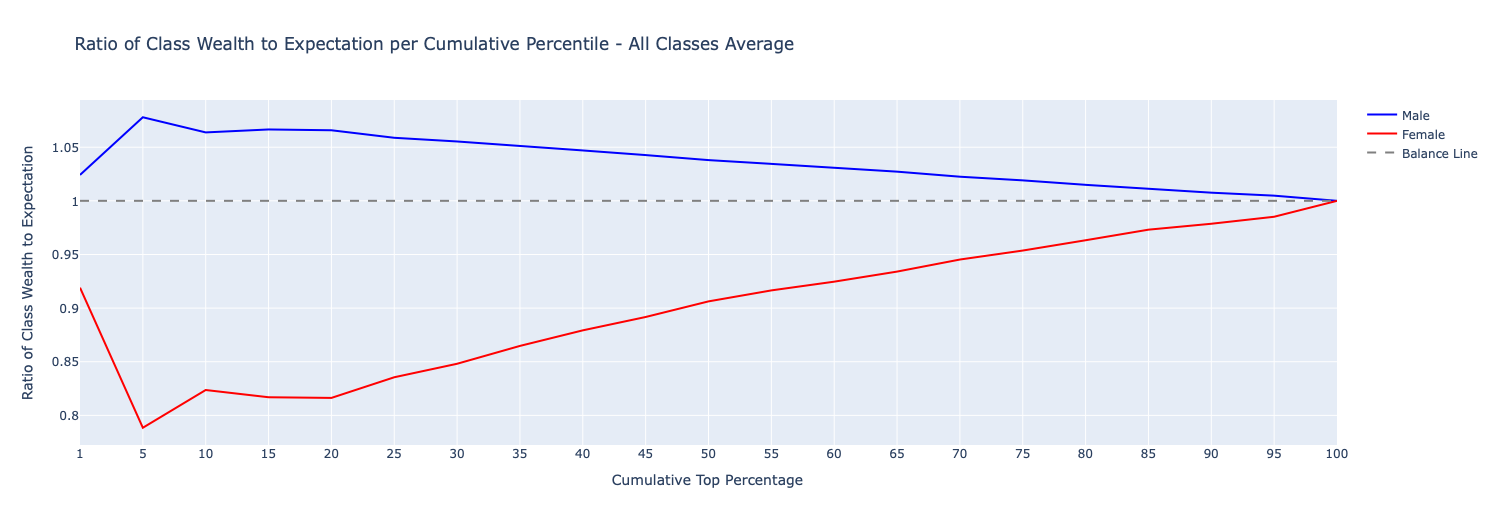
\includegraphics[clip,width=1.0\columnwidth]{Ratio of Class Wealth to Expectation per Cumulative Top Percentage - All Classes Average - Gender}%
}

\subfloat[Ratio of Class Wealth to Expectation per Quantile - All Classes Average\label{fig:test2}]{%
  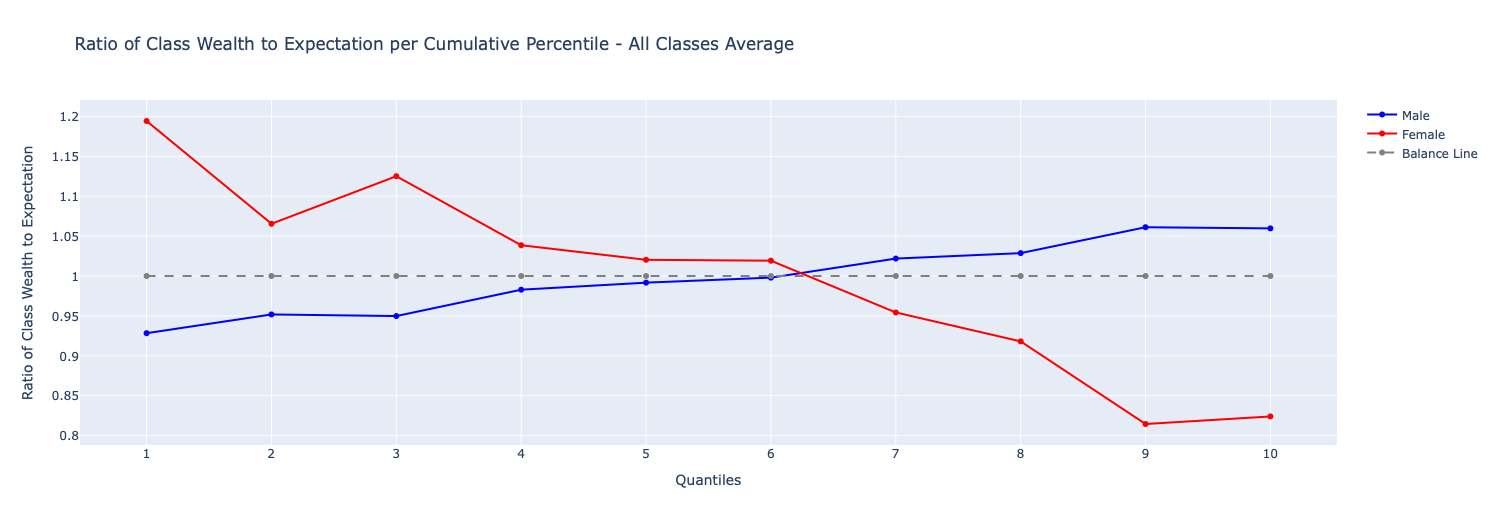
\includegraphics[clip,width=1.0\columnwidth]{Ratio of Class Wealth to Expectation per Quantile - All Classes Average - Gender}%
}

\caption{Ratio of each gender wealth to expectaion} \label{fig:gender - ratio of gender wealth to expectation}

\end{figure}

From \autoref{fig:gender - ratio of gender wealth to expectation} the value of ratio between top \(x\)\% potion to the expectation in the above tables, we can see that on average, the rich entities are dominated by male. Exceptions are held for 3 classes, that is classes American singer, businessperson, and badminton player. Moreover, as we set bigger portions (higher percentage), the gap of ratio between the two ender in each class decreases i.e. the value of top \(x\)\% relative to expectation of both genders converge to 1.
% \paragraph{Western Bias in Wikidata.}
\paragraph{Regional Knowledge Gap: Western vs. Non-Western Representation.}
Regional knowledge gap analysis in Wikidata will be performed on 5 Wikidata classes: computer scientist, singer, memorial, university, and river. For each class, we collected the data for the western portion from 8 countries: Canada, France, Germany, Ireland, Poland, Switzerland, the United Kingdom (UK), and the United State of America (USA). For the non-western portion, we also selected 8 countries: China, Egypt, India, Indonesia, Japan, Morocco, Nigeria, and South Africa. The selected countries represent different continents to capture a diverse geographic distribution. Additionally, we focused on large and well-known countries to ensure the dataset is representative, as data from smaller countries may not provide meaningful insights due to limited coverage in Wikidata.

To analyze the gap, the first aspect that will be considered is the proportion of each regional category in every class. We assumed that there are equal numbers of western and non-western and this will be the basis to determine if there is any gap in the data. Pearson's chi-square test (goodness-of-fit) is then performed to test the null and alternative hypotheses with significance level of \(\alpha=5\%\) as follows:

% \(H_0\): The proportions of western and non-western entities in a particular class are equal

% \(H_1\): The proportions of western and non-western entities in a particular class are not equal

\begin{table}[h]
    \centering
    \renewcommand{\arraystretch}{1.3}
    \begin{tabular}{|l p{12cm}|} 
        \hline
        \multicolumn{2}{|l|}{\textbf{Regional Knowledge Gap: Entity Count Gap (Pearson's chi-square test)}} \\
        \hline
        \textbf{$H_0$} & The proportions of western and non-western entities in a particular class are equal. \\
        \textbf{$H_1$} & The proportions of western and non-western entities in a particular class are not equal. \\
        \hline
        \textbf{Insight 1:} & Across all 5 classes, the proportions of western and non-western entities differ significantly. Western entities dominate in 4 out of 5 classes, with the only exception being the university class, which is skewed toward non-western entities. \\
        \hline
    \end{tabular}
\end{table}

% \vspace{-3em}

\begin{center}
\scriptsize
\begin{threeparttable}
\captionsetup{font=small}
\caption{Entity Count of 5 Wikidata Classes per Regional Category}
\label{tab:western - entity count}
\begin{tabular}{c | c c c c c c c} 

\toprule
    Class Name & Entity & Western & \CellWithForceBreak{Non- \\ western} & \%Western & \CellWithForceBreak{\%Non- \\ western}& $\chi^2$ & p-value \\ [0.5ex] 
\midrule
    Computer scientist & 6063 & 5446 & 617 & 0.90 & 0.10 & 3846.15 & 0.0 \\
    Singer & 43240 & 31039 & 12201 & 0.72 & 0.28 & 8206.99 & 0.0 \\
    Memorial & 4011 & 3836 & 175 & 0.96 & 0.04 & 3341.54 & 0.0 \\
    University & 6124 & 2398 & 3726 & 0.39 & 0.61 & 287.98 & 1.37e-64 \\
    River & 125567 & 70059 & 55508 & 0.56 & 0.44 & 1686.20 & 0.0 \\
    [1ex]
\bottomrule
\end{tabular}
\begin{tablenotes}
    \scriptsize
    \item{This table shows the entity count of 5 Wikidata classes per regional category. Chi-square test result shows the significance of difference between the entity count of the two regions.}
\end{tablenotes}
\end{threeparttable}
\end{center}

From \autoref{tab:western - entity count}, we can observe that the proportion of western entities exceeds that of non-western entities in 4 out of the 5 classes. In the memorial and computer scientist classes, the gap is particularly striking, with western entities making up over 90\% of the total population. Similarly, in the singer and river classes, western entities also represent the majority. The university class is the only exception, where non-western entities slightly outnumber western ones, comprising 61\% of the total. Based on the results of the chi-square test, the p-values in all five classes are well below the significance threshold ($\alpha = 0.05$), leading us to reject the null hypothesis. This indicates that the differences in entity proportions between western and non-western entities are statistically significant and not due to random variation.

However, similar to entity count in gender-based knowledg gap analysis, it is debatable that some of these gaps are expected. For instance, the dominance of western representation in the computer scientist or memorial classes is not necessarily a result of data entry errors or systemic bias within Wikidata alone. Instead, it may mirror general historical and sociopolitical factors, such as unequal access to documentation, global academic visibility, and archival infrastructure. Conversely, the university class, where the number of non-western entities are higher, might be a reflection of population-driven realities, as countries like China, India, and Indonesia possess massive populations and have established a vast number of higher education institutions to serve their demographic needs. The greater number of non-western universities represented in Wikidata is probably a result of this population scale. Due to this, raw entity count alone may not be an ideal measure of gap. To more accurately assess representation and equity, we must consider other metrics that analyze wealth distribution and prominence at the entity level.

% From \autoref{tab:western - central tendency}, non-western entities generally have lower values of measure of central tendency (mean, median, mode). The range of property count of non-westerns is generally also lower than the westerns. Positive values of skewness (skewness > 0) and high kurtosis values (kurtosis > 3) in all classes denote the wealth distribution is right skewed and leptokurtic.

The next step in our analysis is examining the measures of central tendency and dispersion to evaluate where the knowledge wealth is concentrated and how it varies between western and non-western entities.

\begin{table}[h]
    \centering
    \renewcommand{\arraystretch}{1.3}
    \begin{tabular}{|l p{12cm}|} 
        \hline
        \multicolumn{2}{|l|}{\textbf{Regional Knowledge Gap: Measures of Central Tendency and Dispersion}} \\
        \hline
        \textbf{Insight 1:} & In 4 out of 5 classes, western entities have higher mean, median, and mode values than non-western entities, indicating greater concentration of knowledge wealth. \\
        \textbf{Insight 2:} & Western entities generally exhibit higher standard deviations, skewness, and kurtosis, suggesting greater variability, more frequent outliers, and stronger right-skewed distributions. \\
        \hline
    \end{tabular}
\end{table}

% \vspace{-3em}

\begin{center}
\scriptsize
\begin{threeparttable}
\captionsetup{font=small}
\caption{Measures of Central Tendency of 5 Wikidata Classes per Regional Category}
\label{tab:western - central tendency}
\begin{tabular}{c | c c c} 
\toprule
    Class Name & \CellWithForceBreak{Mean \\ (o/w/n)} & \CellWithForceBreak{Median \\ (o/w/n)} & \CellWithForceBreak{Mode \\ (o/w/n)} \\ [0.5ex] 
\midrule
    Computer scientist & 35.00/35.87/27.24 & 29.00/29.00/22.00 & 21/15/16 \\
    Singer & 34.99/39.14/24.43 & 25.00/29.00/18.00 & 15/18/14 \\
    Memorial & 11.04/11.04/11.13 & 9.00/9.00/9.00 & 9/9/9 \\
    University & 23.11/31.61/17.63 & 17.50/24.00/16.00 & 6/6/6 \\
    River & 7.69/8.55/6.60 & 7.00/7.00/6.00 & 7/7/7 \\
    [1ex]
\bottomrule
\end{tabular}
\begin{tablenotes}
    \scriptsize
    \item{This table shows the measures of central tendency of 5 Wikidata classes per regional category. Each measure will have 3 values: o (overall), w (western), and n (non-western).}
\end{tablenotes}
\end{threeparttable}
\end{center}

% \vspace{-2em}

\begin{center}
\scriptsize
\begin{threeparttable}
\captionsetup{font=small}
\caption{Measures of Dispersion and Symmetry of 5 Wikidata Classes per Regional Category}
\label{tab:western - dispersion and symmetry}
\begin{tabular}{c | c c c c c} 

\toprule
    Class Name & \CellWithForceBreak{Min \\ (o/w/n)} & \CellWithForceBreak{Max \\ (o/w/n)} & \CellWithForceBreak{Std. Deviation \\ (o/w/n)} & \CellWithForceBreak{Skewness \\ (o/w/n)} & \CellWithForceBreak{Kurtosis \\ (o/w/n)} \\ [0.5ex] 
\midrule
    Computer scientist & 4/4/5 & 441/441/145 & 25.15/25.67/18.15 & 3.02/3.02/2.37 & 20.90/20.83/8.49 \\
    Singer & 3/4/3 & 687/687/379 & 33.27/36.60/18.94 & 4.49/4.28/3.15 & 35.56/31.09/21.59 \\
    Memorial & 2/3/2 & 142/142/52 & 5.89/5.82/7.28 & 8.50/8.95/2.98 & 143.57/156.15/12.79 \\
    University & 2/2/2 & 234/234/166 & 20.00/25.88/12.25 & 2.37/1.65/2.22 & 10.34/5.33/12.70 \\
    River & 2/2/2 & 452/452/148 & 5.24/6.46/2.68 & 21.71/19.54/14.67 & 1152.84/868.56/465.42 \\
    [1ex]
\bottomrule
\end{tabular}
\begin{tablenotes}
    \scriptsize
    \item{This table shows the measures of dispersion and symmetry of 5 Wikidata classes per regional category. Each measure will have 3 values: o (overall), w (western), and n (non-western).}
\end{tablenotes}
\end{threeparttable}
\end{center}

From \autoref{tab:western - central tendency}, we observed that in 4 out of 5 classes, western entities consistently show higher values across all measures of central tendency (mean, median, and mode) compared to non-western entities. This suggests that western entities tend to be richer in knowledge wealth. The memorial class is the only exception, where both groups exhibit nearly identical values. A particularly extreme disparity is observed in the university class, where the mean property count for western entities (31.61) is nearly double that of non-western entities (17.63), highlighting a strong central tendency skew. This extreme pattern can also be seen in the singer class.

Turning to the measures of dispersion and symmetry in \autoref{tab:western - dispersion and symmetry}, we saw that standard deviation is generally higher for western entities across all classes except memorial, suggesting greater wealth variability among western entities. Furthermore, in the university class, western entities show a standard deviation of 25.88, more than double that of non-western entities at 12.25. We also observed positive skewness and high kurtosis across all classes and both regions, indicating that knowledge wealth distributions are right-skewed and leptokurtic. However, western entities often exhibit higher values, implying more extreme outliers and longer tails. For example, in the river class, the skewness and kurtosis for western entities are 19.54 and 868.56, respectively, compared to 14.67 and 465.42 for non-western entities.

Taken together, these statistics suggest that western entities tend not only to accumulate more knowledge wealth on average but also to dominate the extreme high end of the distribution. In contrast, non-western entities tend to cluster around lower values with tighter distribution, reinforcing regional disparity in knowledge representation.

At a glance, western entities appear to be richer compared to their non-western counterparts. To statistically verify this, we conducted a series of mean comparison tests between the two groups. We began by applying the F-test to assess whether the western and non-western subsets within each class have equal variance. The result of the F-test determines the appropriate test to be used: if the p-value is greater than 0.05, indicating equal variance, we use the standard t-test; otherwise, we apply Welch's test, which does not assume equal variance.

% Out of 5 classes, class of memorial is the only class where the null hypothesis is not rejected. In the other 4 classes, we can see a significant difference between the mean of the two reginal categories, which all are in favor of the western.

\begin{table}[h!]
    \centering
    \renewcommand{\arraystretch}{1.3}
    \begin{tabular}{|l p{12cm}|} 
        \hline
        \multicolumn{2}{|l|}{\textbf{Regional Knowledge Gap: Mean of Wealth Gap (two-sided t-test and Welch's test)}} \\
        \hline
        \textbf{$H_0$} & The means of wealth of western and non-western entities in a particular class are equal. \\
        \textbf{$H_1$} & The means of wealth of western and non-western entities in a particular class are not equal. \\
        \hline
        \textbf{Insight 1:} & In 4 out of 5 classes, western entities have significantly higher mean knowledge wealth than non-western entities. \\
        \hline
    \end{tabular}
\end{table}

% \vspace{-3em}

\begin{center}
\scriptsize
\begin{threeparttable}
\captionsetup{font=small}
\caption{F-Test, T-Test, and Welch's Test Result of 5 Wikidata Classes}
\label{tab:western - mean test}
\begin{tabular}{c | c c c c c c} 
\toprule
    Class Name & \CellWithForceBreak{F-Test \\ statistic} & \CellWithForceBreak{F-Test \\ p-value} & \CellWithForceBreak{T-Test \\ statistic} & \CellWithForceBreak{T-Test \\ p-value} & \CellWithForceBreak{Welch's Test \\ statistic} & \CellWithForceBreak{Welch's \\ p-value} \\ [0.5ex] 
\midrule
    Computer scientist & 2.00 & 1.00 & 8.13 & 5.10e-16 & - & - \\
    Singer & 3.73 & 1.00 & 42.22 & 0.0 & - & - \\
    Memorial & 0.64 & 0.00 & - & - & -0.16 & 0.88 \\
    University & 4.46 & 1.00 & 28.40 & 8.23e-167 & - & - \\
    River & 5.83 & 1.00 & 66.91 & 0.0 & - & - \\
 [1ex]
\bottomrule
\end{tabular}
\begin{tablenotes}
    \scriptsize
    \item{}
\end{tablenotes}
\end{threeparttable}
\end{center}

The result of the F-test in \autoref{tab:western - mean test} shows that only one class, that is, memorial, has unequal variance (p < 0.05), thus requiring the use of Welch's test. For the remaining four classes, the t-test was applied. From the test results, we rejected the null hypothesis in 4 out of 5 classes, indicating that the difference in mean wealth between western and non-western entities is statistically significant. The only exception is the memorial class, where Welch's test yields a p-value of 0.88, suggesting no significant difference in mean. Among the classes with significant results, the direction of difference consistently favors Western entities. This can be seen clearly in classes such as university and singer, where the t-statistics are noticeably high (28.40 and 42.22, respectively) and the p-values are zero. These findings align with our previous observations that western entities dominate in terms of quantity and average information richness. We conclude that western entities are more likely to have higher mean knowledge wealth than non-western ones, although exceptions like the memorial class suggest that certain domains may present a more balanced knowledge distribution.

As with gender-based knowledge gap, measuring regional gap in Wikidata cannot rely solely on entity counts. The number of entities associated with western and non-western regions may reflect real-world disparities in documentation or notability, making raw counts an unreliable indicator of gap. Similarly, measures of central tendency, such as the mean or median, fail to capture how representation is distributed across the full spectrum of prominence or wealth. To address these limitations, we applied the same metric introduced in the gender-based gap analysis: the relative expectation ratio. This measure compares a region's share of entities within a given quantile to its expected share under equal representation. A ratio of 1 indicates proportional representation, while values above or below 1 signal overrepresentation or underrepresentation, respectively. This allows for a more nuanced, quantile-level understanding of how western and non-western entities are distributed in knowledge graphs like Wikidata.

\begin{table}[h]
    \centering
    \renewcommand{\arraystretch}{1.3}
    \begin{tabular}{|l p{12cm}|} 
        \hline
        \multicolumn{2}{|l|}{\textbf{Regional Knowledge Gap: Relative Expectation Ratios}} \\
        \hline
        \textbf{Insight 1:} & On average across all 5 classes, the less prominent segments are dominated by non-western entities, while the more prominent ones are dominated by western entities. The middle quantiles exhibit a zig-zag pattern, reflecting inconsistent representation between the two groups. \\
        \textbf{Insight 2:} & At the individual class level, 2 out of 5 classes display a particularly strong western dominance. The rests exhibit a zig-zag trend. \\
        \hline
    \end{tabular}
\end{table}

On average across all classes, the lower four quantiles (i.e., the less prominent or "poorer" segments) are predominantly composed of non-western entities, while the top three quantiles (i.e., the more prominent or "wealthier" segments) are dominated by western entities. The middle quantiles exhibit a zig-zag pattern, reflecting inconsistent representation between the two groups. At the individual class level, the computer scientist and singer classes display a particularly strong western bias. In both classes, non-western entities are consistently overrepresented in the lower quantiles (Q1–Q4), while western entities are consistently overrepresented in the upper quantiles (Q5–Q6). This pattern suggests a clear stratification, with non-western entities disproportionately concentrated in less prominent positions. The memorial, university, and river classes, however, deviate from this pattern and exhibit a zig-zag trend across quantiles. This suggests a more unstable distribution of western and non-western entities across the quantiles.

\begin{figure}
\centering 
\subfloat[Ratio of Class Wealth to Expectation per Cumulative Top Percentage - All Classes Average
\label{fig:test1 - western}]{%
  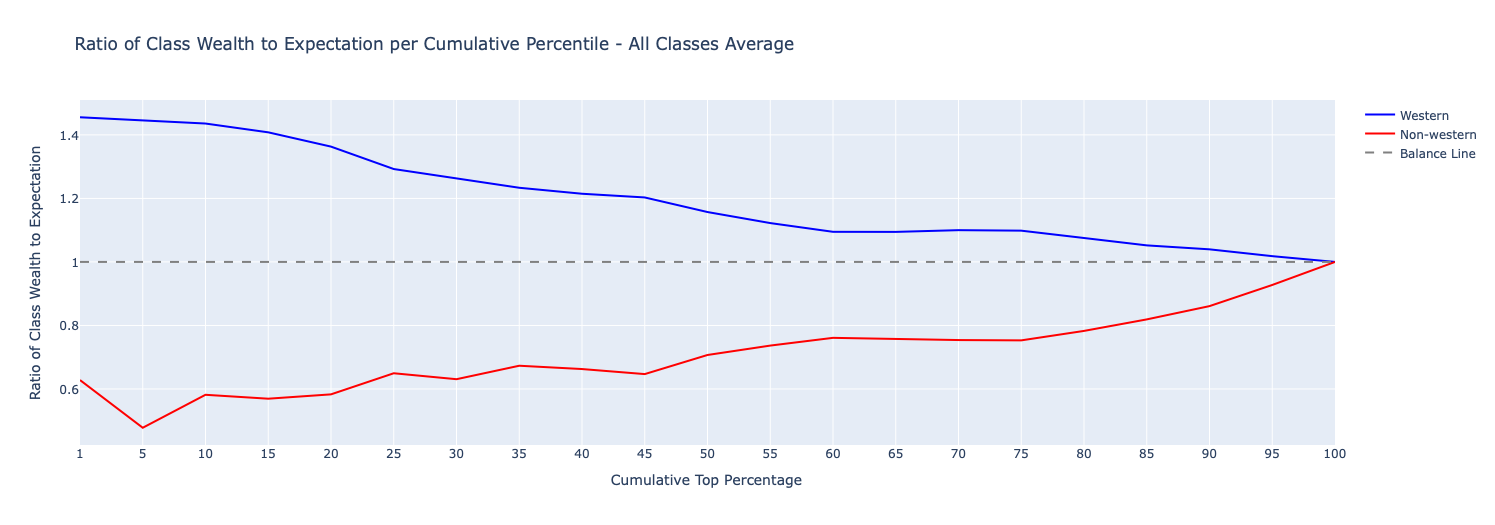
\includegraphics[clip,width=1.0\columnwidth]{Ratio of Class Wealth to Expectation per Cumulative Top Percentage - All Classes Average - Region}%
}

\subfloat[Ratio of Class Wealth to Expectation per Quantile - All Classes Average\label{fig:test2 - western}]{%
  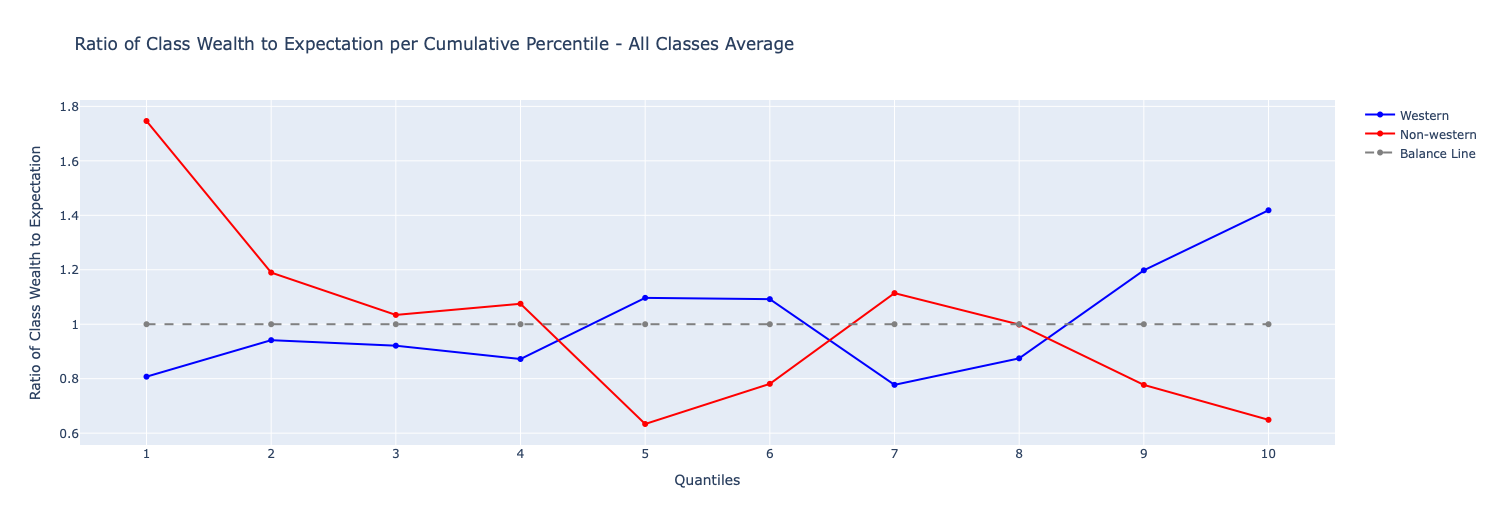
\includegraphics[clip,width=1.0\columnwidth]{Ratio of Class Wealth to Expectation per Quantile - All Classes Average - Gender - Region}%
}

\caption{Ratio of each regional wealth to expectation}\label{fig:western - ratio of regional wealth to expectation}

\end{figure}
\subsection{Effect of Type of Wealth on Inequality Measure} \label{wealth & gini}

% \begin{center}
    \small
    \begin{threeparttable}
    \caption{Gini Bag-Set}
    \label{tab:gini bag-set}
    \begin{tabular}{c c c} 
    
    \toprule
        Class Name & Gini Bag & Gini Set \\ [0.5ex] 
    \midrule
        Historical painting & 0.22 & 0.14 \\
        University & 0.44 & 0.41 \\
        Sci-fi book & 0.32 & 0.22 \\
        Memorial & 0.22 & 0.18 \\
        American researcher & 0.33 & 0.31 \\
        American singer & 0.40 & 0.39 \\
        Badminton player & 0.29 & 0.14 \\
        Computer scientist & 0.41 & 0.37 \\
        [1ex]
    \bottomrule
    \end{tabular}
    \begin{tablenotes}
        \footnotesize
        This table shows the measures of gini coefficient of knowledge wealth based on the (non-)uniqueness of individual properties of 8 Wikidata classes
    \end{tablenotes}
    \end{threeparttable}
\end{center}
% \begin{center}
    \small
    \begin{threeparttable}
    \caption{Gini Object-Literal-ID}
    \label{tab:gini proptype}
    \begin{tabular}{c c c c} 
    
    \toprule
        Class Name & Gini Object & Gini Literal & Gini ID \\ [0.5ex] 
    \midrule
        American researcher & 0.26 & 0.50 & 0.50 \\
        American singer & 0.29 & 0.50 & 0.53 \\
        Badminton player & 0.30 & 0.36 & 0.60 \\
        Computer scientist & 0.36 & 0.54 & 0.56 \\
        Historical painting & 0.25 & 0.27 & 0.44 \\
        Memorial & 0.20 & 0.30 & 0.40 \\
        Sci-fi book & 0.35 & 0.34 & 0.42 \\
        University & 0.40 & 0.49 & 0.53 \\
        [1ex]
    \bottomrule
    \end{tabular}
    \begin{tablenotes}
        \footnotesize
        This table shows the measures of gini coefficient of knowledge wealth based on types of property of 8 Wikidata classes
    \end{tablenotes}
    \end{threeparttable}
\end{center}
% \begin{center}
    \small
    \begin{threeparttable}
    \caption{Gini Outgoing-Incoming}
    \label{tab:gini outgoing-incoming}
    \begin{tabular}{c c c} 
    
    \toprule
        Class Name & Gini Outgoing & Gini Incoming \\ [0.5ex] 
    \midrule
        Historical painting & 0.22 & 0.86 \\
        University & 0.44 & 0.91 \\
        Sci-fi book & 0.32 & 0.82 \\
        Memorial & 0.22 & 0.99 \\
        American researcher & 0.33 & 0.77 \\
        American singer & 0.40 & 0.82 \\
        Badminton player & 0.29 & 0.68 \\
        Computer scientist & 0.41 & 0.81 \\
        [1ex]
    \bottomrule
    \end{tabular}
    \begin{tablenotes}
        \footnotesize
        This table shows the measures of gini coefficient of knowledge wealth based on the direction of link of 8 Wikidata classes
    \end{tablenotes}
    \end{threeparttable}
\end{center}

In this subchapter, analysis is done to see how each wealth type affects the level of inequality of Wikidata classes. There are 2 ways this is done--quantitatively using Gini coefficient and qualitatively using Lorenz curve. The analysis is performed on 8 Wikidata classes, in which 4 of them are human-related class while the other 4 are not.

When looking at the notion of wealth using the characteristics of (non-)uniqueness of individual properties, it is intuitive that the measure of bag of properties will always give higher (or at least, equal) amount of wealth compared to the measure of set. Set of property will have an upper bound of number of unique property, while bag of properties does not have any upper bound. Moreover, using bag of properties, a large number of triples having the same property may inflate the wealth substantially--though this is not necessarily a problem nor an advantage. This characteristics has a direct impact on inequality measure and it is well depicted on the value of Gini coefficient. From \autoref{table:gini-coef}, in all clasess, the Gini coefficient using bag of properties is always higher than of set of properties.

% - object, literal, ID: object tends to have lower inequality
Using the notion of wealth by type of property, in general the smallest Gini coefficient value is mostly from wealth using object property. The second one is when using literal, while the biggest one always comes when using ID.

% - outgoing, incoming: incoming shows very high Gini, this is because it is harder --> show the lorenz curve
Using the notion of wealth by the direction of the link, the Gini coefficient when using incoming link is always higher than using outgoing link. By inspecting the Lorenz curve, we can see that most entities do not have any incoming link, and only the small percentage of entites has some incoming link. \autoref{fig:gini-outgoin&incoming} shows the comparison of Lorenz curve of knowledge wealth based on the direction of the link from 3 Wikidata classes. The difference between the two is very significant, because in \autoref{fig:gini-outgoing} the Lorenz curves are closer to the perfect equality line, meanwhile in \autoref{fig:gini-incoming} the diagonal and the Lorenz curve almost form a right triangle which is very close to maximum inequality.

% add to discussion 
% - Wikidata = entity-centric knowledge graph, dimana bentuknya (s,p,o) dengan s sebagai subject of interest. jadi memang expected bahwa outgoing banyak 
% sedangkan incoming mostly justru 0.
% - sedrastis ini perbedaan incoming vs outgoing. incoming link is underestimated. given o, what is the (s, p)
% - kasih contoh: 2 entitas yang secara outgoing mirip, tapi incoming-nya jomplang (1 kaya 1 miskin)

\begin{center}
    \small
    \begin{threeparttable}
    \caption{Knowledge Wealth Type on Gini Coefficient}
    \label{table:gini-coef}
    \begin{tabular}{c | c c | c c c | c c} 
    
    \toprule
        Class Name & \CellWithForceBreak{Gini \\ Bag} & \CellWithForceBreak{Gini \\ Set} & \CellWithForceBreak{Gini \\ Object} & \CellWithForceBreak{Gini \\ Literal} & \CellWithForceBreak{Gini \\ ID} & \CellWithForceBreak{Gini \\ Outgoing} & \CellWithForceBreak{Gini \\ Incoming} \\ [0.5ex] 
    \midrule
        American researcher & 0.33 & 0.31 & 0.25 & 0.27 & 0.44 & 0.33 & 0.77 \\
        American singer & 0.40 & 0.39 & 0.20 & 0.30 & 0.40 & 0.40 & 0.82 \\
        Badminton player & 0.29 & 0.14 & 0.35 & 0.34 & 0.42 & 0.29 & 0.68 \\
        Computer scientist & 0.41 & 0.37 & 0.40 & 0.49 & 0.53 & 0.41 & 0.81 \\
        Memorial & 0.22 & 0.18 & 0.36 & 0.54 & 0.56 & 0.22 & 0.99 \\
        Historical painting & 0.22 & 0.14 & 0.26 & 0.50 & 0.50 & 0.22 & 0.86 \\
        Sci-fi book & 0.32 & 0.22 & 0.30 & 0.36 & 0.60 & 0.32 & 0.82 \\
        University & 0.44 & 0.41 & 0.29 & 0.50 & 0.53 & 0.44 & 0.91 \\
        [1ex]
    \bottomrule
    \end{tabular}
    \begin{tablenotes}
        \footnotesize
        \item{This table shows the comparison of Gini coefficient of 8 Wikidata classes}
    \end{tablenotes}
    \end{threeparttable}
\end{center}

\begin{figure}[!h]
    \centering 
    \subfloat[Lorenz curve of wealth using outgoing link
    \label{fig:gini-outgoing}]{%
      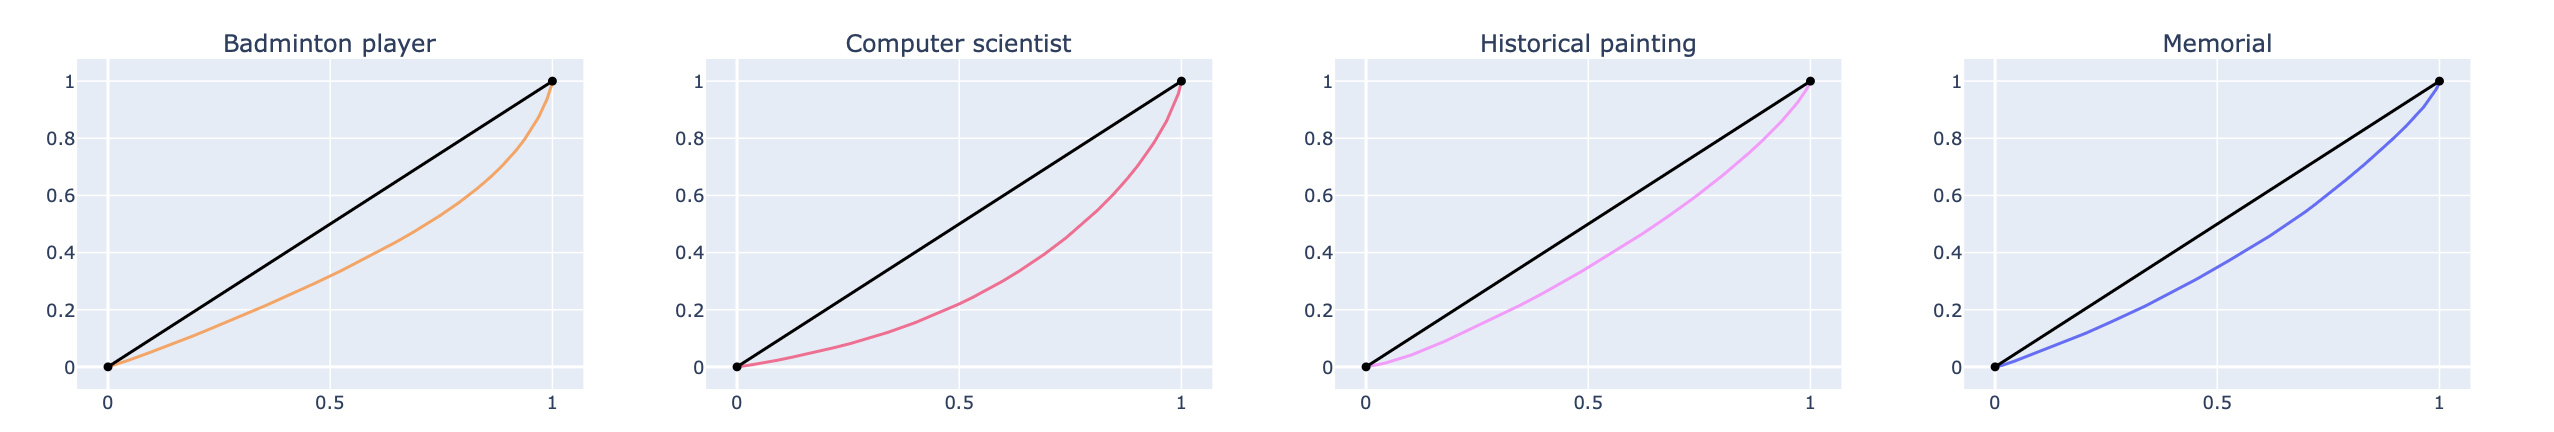
\includegraphics[clip,width=1.0\columnwidth]{Gini - Outgoing}%
    }
    
    \subfloat[Lorenz curve of wealth using incoming link\label{fig:gini-incoming}]{%
      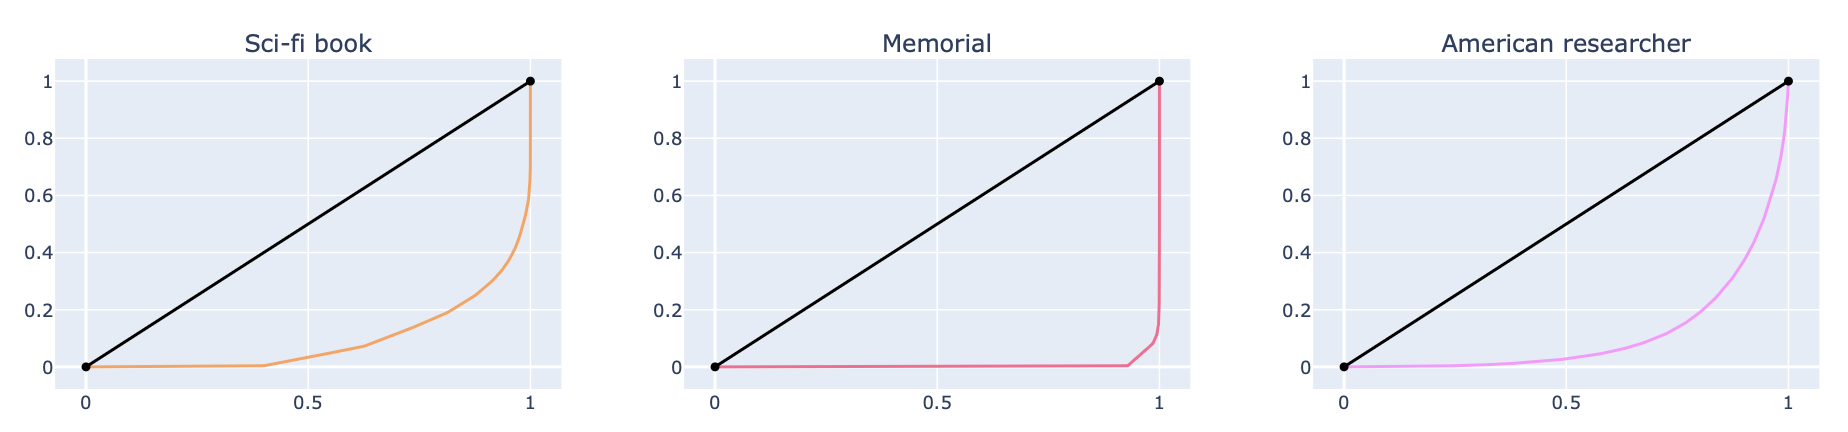
\includegraphics[clip,width=1.0\columnwidth]{Gini - Incoming.png}%
    }
    
    \caption{Comparison of Lorenz curve of wealth based on the direction of link} \label{fig:gini-outgoin&incoming}
    
\end{figure}
\subsection{Contribution of Property Type to Knowledge Wealth} \label{wealth & proptype contribution}

In this subchapter, analysis is done to see how much contribution of each property types to the knowledge wealth of Wikidata classes. The analysis is performed on 8 Wikidata classes, in which 4 of them are human-related class while the other 4 are not. The wealth of each classes is calculated using the concept of bag of properties and set of properties, for each property types (object, literal, ID, and their combinations).

Two methods of averaging are used in this analysis—global percentage and average contribution per individual entity. The first method is done by calculating the total sum of each property across all entities and then dividing it by the grand total of all properties combined, providing a holistic view of each property's overall contribution. The second method is done by first determining the percentage contribution of each property within each individual entity and then averaging these percentages across all entities, ensuring that every entity is equally represented regardless of its scale. While the global percentage method highlights absolute contributions, the average per-entity method captures relative contributions within each entity, making it more robust to variations in scale.

\begin{center}
    \small
    \makebox[\linewidth]{
    \begin{threeparttable}
    \caption{Contribution of Property Type to Knowledge Wealth Using Bag of Properties}
    \label{table:prop-contribution-bag}
    \begin{tabular}{c | c c c | c | c} 
    
    \toprule
        Class Name & \CellWithForceBreak{\% Object \\ Bag} & \CellWithForceBreak{\% Literal \\ Bag} & \CellWithForceBreak{\% ID \\ Bag} & \CellWithForceBreak{\% Literal + ID \\ Bag} & \CellWithForceBreak{\% Object + Literal \\ Bag} \\ [0.5ex] 
    \midrule
        American researcher & 59.55 / 65.65 & 3.32 / 2.8 & 37.12 / 31.55 & 40.45 / 34.35 & 62.88 / 68.45 \\
        American singer & 40.44 / 48.42 & 7.47 / 8.48 & 52.09 / 43.1 & 59.56 / 51.58 & 47.91 / 56.9 \\
        Badminton player & 79.34 / 78.96 & 10.14 / 11.68 & 10.52 / 9.36 & 20.66 / 21.04 & 89.48 / 90.64 \\
        Computer scientist & 59.36 / 65.93 & 4.19 / 3.71 & 36.44 / 30.36 & 40.64 / 34.07 & 63.56 / 69.64 \\
        Historical painting & 66.35 / 66.46 & 25.48 / 25.85 & 8.17 / 7.69 & 33.65 / 33.54 & 91.83 / 92.31 \\
        Memorial & 62.82 / 64.16 & 21.0 / 20.4 & 16.18 / 15.44 & 37.18 / 35.84 & 83.82 / 84.56 \\
        Sci-fi book & 62.96 / 62.62 & 14.44 / 15.78 & 22.59 / 21.6 & 37.04 / 37.38 & 77.41 / 78.4 \\
        University & 37.59 / 44.79 & 18.11 / 18.31 & 44.3 / 36.9 & 62.41 / 55.21 & 55.7 / 63.1 \\
        [1ex]
    \bottomrule
    \end{tabular}
    \begin{tablenotes}
        \footnotesize
        \item{This table shows the contribution of each property type of 8 Wikidata classes based on the notion of bag of properties. Each record has 2 values separated by "/". The first value is the contribution rate when calculated with global percentage method, and the second one is when using the average contribution per individual entity}
    \end{tablenotes}
    \end{threeparttable}
    }
\end{center}

\begin{center}
    \small
    \makebox[\linewidth]{
    \begin{threeparttable}
    \caption{Contribution of Property Type to Knowledge Wealth Using Set of Properties}
    \label{table:prop-contribution-set}
    \begin{tabular}{c | c c c | c | c} 
    
    \toprule
        Class Name & \CellWithForceBreak{\% Object \\ Set} & \CellWithForceBreak{\% Literal \\ Set} & \CellWithForceBreak{\% ID \\ Set} & \CellWithForceBreak{\% Literal + ID \\ Set} & \CellWithForceBreak{\% Object + Literal \\ Set} \\ [0.5ex] 
    \midrule
        American researcher & 51.25 / 59.69 & 3.97 / 3.29 & 44.78 / 37.02 & 48.75 / 40.31 & 55.22 / 62.98 \\
        American singer & 33.91 / 43.58 & 8.1 / 9.18 & 57.99 / 47.24 & 66.09 / 56.42 & 42.01 / 52.76 \\
        Badminton player & 71.75 / 74.13 & 13.79 / 13.9 & 14.46 / 11.97 & 28.25 / 25.87 & 85.54 / 88.03 \\
        Computer scientist & 50.53 / 60.54 & 4.98 / 4.27 & 44.49 / 35.19 & 49.47 / 39.46 & 55.51 / 64.81 \\
        Historical painting & 60.57 / 61.91 & 28.88 / 28.61 & 10.55 / 9.48 & 39.43 / 38.09 & 89.45 / 90.52 \\
        Memorial & 60.06 / 62.01 & 22.41 / 21.59 & 17.54 / 16.4 & 39.94 / 37.99 & 82.46 / 83.6 \\
        Sci-fi book & 59.36 / 61.91 & 13.86 / 14.59 & 26.78 / 23.5 & 40.64 / 38.09 & 73.22 / 76.5 \\
        University & 33.93 / 42.74 & 17.67 / 18.32 & 48.4 / 38.95 & 66.07 / 57.26 & 51.6 / 61.05 \\
        [1ex]
    \bottomrule
    \end{tabular}
    \begin{tablenotes}
        \footnotesize
        \item{This table shows the contribution of each property type of 8 Wikidata classes based on the notion of set of properties. Each record has 2 values separated by "/". The first value is the contribution rate when calculated with global percentage method, and the second one is when using the average contribution per individual entity}
    \end{tablenotes}
    \end{threeparttable}
    }
\end{center}

From \autoref{table:gini-coef} 
When we look at the contribution of each type of property to the overall wealth, ....
Overall, the usage of pure literal properties is lower than of object and ID. This aligns with the principle of knowledge graph to use URI for internal connections and ID for external resources.


% \subsection{(Tentative)Proxy of Knowledge Wealth: Real-World Rankings}
% - Popularity
% - Movie IMDb
% - GDP, economic wealth
% - Personal net worth

% \subsection{(Tentative) Basics of Knowledge Wealth Comparison}

% \paragraph{Subclass-to-Subclass Wealth Comparison}
% \paragraph{Subclass-to-Superclass Wealth Comparison}
% \paragraph{Totally Different Classes Wealth Comparison}

% \subsection{(Tentative) Knowledge Wealth Evolution using Wikidata History}

% \subsection{(Tentative) Pareto Principle in Wikidata}

% \subsection{(Tentative)}
% This is additional, if possible. Based on WN notes to use statistical measures for machine learning

\section{Discussion}

% add to discussion 
% - Wikidata = entity-centric knowledge graph, dimana bentuknya (s,p,o) dengan s sebagai subject of interest. jadi memang expected bahwa outgoing banyak 
% sedangkan incoming mostly justru 0.
% - sedrastis ini perbedaan incoming vs outgoing. incoming link is underestimated. given o, what is the (s, p)
% - kasih contoh: 2 entitas yang secara outgoing mirip, tapi incoming-nya jomplang (1 kaya 1 miskin)
\paragraph{Generality of Framework}
The framework that is proposed in this study is applicable to any kind of knowledge graph. However, the library that we built for experimentation is specifically for Wikidata, because the query service, structure, and response is very unique for each knowledge graph. If further experimentation is to be conducted for other knowledge graph, then the library needs to be modified.

\paragraph{Issue of Incoming Link}
Wikidata is an entity-centric knowledge graph which means in the editathon efforts, the subject \(s\) is always be the subject of interest and the starting point to be edited by contributors. It is very unlikely that the opposite approach is done, that is, an object \((o)\) is given and a pair subject and property \((s, p)\) is to be searched. Not only from the contributors, the platform itself does not support the later view. This explains the phenomenon that we observed in \autoref{wealth & gini} regarding outgoing and incoming link. With existing subject-centric point of view, the number of new outgoing link introduced to the knowledge graph will grow in a much higher rate as opposed to incoming link. As a result, incoming link will be very rare, or even only present in certain entites.

\paragraph{Weight of Property}
%Content dump for weighted form

% It is intuitive that the measure of bag of properties will always give higher (or at least, equal) amount of wealth compared to the measure of set. Set of property will have an upper bound of number of unique property, while bag of property does not have any upper bound. Moreover, using bag of properties, a large number of triples having the same property may inflate the wealth substantially--though this is not necessarily a problem nor an advantage.

Set of properties might be more suitable if the main concern is the presence of properties, instead of the abundance of information it contains. We will take \textit{WilliamShakespeare} (Q692) in Wikidata as an example. It is reasonable if property like  \textit{date of birth} (P569) to be treated using set of properties, but for a well-known playwright and poet, we shall expect the property \textit{notable work} (P800) to incorporate all or most of his well-known works. If only few works registered in \(G\) despite he has dozens of works, then we might conclude the entity is poor. For this case, treating the property using the notion of set is not preferable because it will fail to capture the aforementioned poor condition, while blatantly using bag of properties might skew the wealth amount.

Due to this, the notion of (non-)uniqueness can be extended to a weighted form. The weight is given independently for each property and can be defined in such a way that is most appropriate for the nature of the property. Example of weight is inverse of median of property count of each entity.

Let \(h_{p_i}\) be the weight of property \(p_i\) in graph \(G\). Let \(N_{bag}(s,G,p_i)\) be a set that comprises all pair  \((p_i,o)\), that is, property \(p_i\) and an object \(o\) that is connected to \(s\). Then \(W_{weighted}(s, G)\) is the sum of \(N_{bag}(s,G,p_i)\) multiplied by the associated weight \(h_{p_i}\).

% \textit{how can we formalize wi to be the function of set(amount of pi in class C in G)??}

% \[
%     \forall p_i, h_i = f_i(....)
% \]
\[
    N_{bag}(s,G,p_i) = \{(p_i, o) | (s, p_i, o) \in G\}
\]
\[
    W_{weighted}(s, G) = \sum_i |N_{bag}(s,G,p_i)| * h_{p_i}
\]

Using \autoref{fig:wealth-weighted}, we can show how the notion of weighted wealth can be calculated. Let's define \(h_{p_1} = 1/median\) and \(h_{p_2} = 1\). For property \(p_1\), \(\{1, 2, 2, 4\}\) is the sorted amount of information contributed from \(p_1\) in each individual entity from \(s_1\) to \(s_4\), from which we get \(h_{p_1} = 1/median = 1/2\). With the above definition, \(W_{weighted}(s_1, G) = 2\), \(W_{weighted}(s_2, G) = 2\), \(W_{weighted}(s_3, G) = 3.5\), \(W_{weighted}(s_4, G) = 1.5\).

Another phenomena that should also be considered is that an entity might have several occurrences of the same property, but this property might just be 'trivial'. This is similar to a document having a lot of 'the' or 'a' (stopwords). Conversely, an entity might just have a single occurrence of a property, but it is a non-trivial one. Perhaps, the property is a highly relevant one for the entity's class. For example, \textit{timePeriod} (P2348) for \textit{William Shakespeare} (Q692) will be a highly relevant one for prominent poets. However, the property \textit{sibling} (P3373) might not be too relevant for Shakespeare's career. One idea to handle such trivial is to regard those porperties using the notion of set of properties--thus we care only on its existence rather than its actual count--or, we can use threshold function to set a tolerance for how much of such trivial we allow.

% =====> OR (alternative of weighted, or generalized form of Wealth based on the (non-)uniqueness of individual properties)

% =====> \(T_i\) is a multiset \(T_i = ... \) -> isinya list semua kontribusi wealth dari property \(p_i\) pada seluruh entity \(S\) pada class \(C\) di graph \(G\) -> keuntungannya disini kita jadi bisa punya fungsi konstan, sehingga bisa catter definisi set, bag, dan weighted secara bersamaan.

Thus, the notion of (non-)uniqueness can be generalized to accommodate the bag, set, and weighted concept. Let \(s_1\), \(s_2\), ... \(s_m\) be \(m\) distinct entities in graph \(G\), which all of them collectively create a class \(C\). Let \(N_{bag}(s,G,p_i)\) be a set that comprises all pair of a particular property \(p_i\) and object, \((p_i,o)\), that is connected to \(s\). We define \(T_{C,p_i}\) a multiset consisted of the number of non-unique properties of each entity of \(C\) contributed from property \(p_i\), i.e., multiset of cardinality of \(N_{bag}(s,G,p_i)\) for all \(s\) in \(C\). For each \(p_i\), let \(f_{p_i}\) be a multivariate function with 2 arguments: \(T_{C,p_i}\) and \(N_{bag}(s,G,p_i)\). \(w_{p_i}\) is the amount of wealth of \(s\) attributed from property \(p_i\), which is calculated by function \(f_{p_i}\). Then \(W_{}(s, G)\) is the sum of \(w_{p_i}\).


\[
    N_{bag}(s,G,p_i) = \{(p_i,o) | (s_j, p_i, o) \in G\}
\]
\[
    T_{C,p_i} = \{|N_{bag}(s,G,p_i)|\ | s \in C\}
\]
\[
    w_{p_i} = f_{p_i}(T_{C,p_i}, |N_{bag}(s,G,p_i)|)
\]
\[
    W_{}(s, G) = \sum_i w_{p_i}
\]

Using \autoref{fig:wealth-weighted}, we can show how the generalized form can be utilized. From the definition, we get \(T_{C,p_1} = \{2, 2, 5, 1\}\) and \(T_{C,p_2} = \{1, 1, 1, 1\}\). Property \(p_1\) illustrates the former issue of trivial. Here, we define $f_{p_1}(x,y) = \begin{cases}
      x & \text{if }x \leq 1 \\
      \frac{x}{2} + 1 & \text{if }1 < x \leq 4 \\
      3 & \text{if }x > 4
    \end{cases}\, $.
For \(p_2\), we want to handle it using the notion of set of properties, thus we define it using a constant function \(f_{p_2}(x,y) = 1\).
With the above definition, \(W_{}(s_1, G) = 3\), \(W_{}(s_2, G) = 3\), \(W_{}(s_3, G) = 4\), \(W_{}(s_4, G) = 2\).

\section{Conclusions}

TBD

\begin{acknowledgments}

TBD

\end{acknowledgments}

\bibliography{mybibliography}

\end{document}